%%%%%%%% ICML 2025 EXAMPLE LATEX SUBMISSION FILE %%%%%%%%%%%%%%%%%

\documentclass{article}
% Recommended, but optional, packages for figures and better typesetting:
\usepackage{microtype}
\usepackage{pdflscape} % Enables landscape pages

% Comment out the following line for the final version to render images 
%\usepackage{graphicx}
\usepackage[draft]{graphicx}

\usepackage{booktabs} % for professional tables
\usepackage{placeins} % Add this to your preamble
\usepackage{tabularx}  % For full-width tables
\usepackage{svg}

% hyperref makes hyperlinks in the resulting PDF.
% If your build breaks (sometimes temporarily if a hyperlink spans a page)
% please comment out the following usepackage line and replace
% \usepackage{icml2025} with \usepackage[nohyperref]{icml2025} above.
\usepackage{hyperref}


% Attempt to make hyperref and algorithmic work together better:
\newcommand{\theHalgorithm}{\arabic{algorithm}}

% Use the following line for the initial blind version submitted for review:
\usepackage{icml2025}

% If accepted, instead use the following line for the camera-ready submission:
% \usepackage[accepted]{icml2025}

% For theorems and such
\usepackage{amsmath}
\usepackage{amssymb}
\usepackage{mathtools}
\usepackage{amsthm}
\usepackage{subcaption}

% if you use cleveref..
\usepackage[capitalize,noabbrev]{cleveref}

%%%%%%%%%%%%%%%%%%%%%%%%%%%%%%%%
% THEOREMS
%%%%%%%%%%%%%%%%%%%%%%%%%%%%%%%%
\theoremstyle{plain}
\newtheorem{theorem}{Theorem}[section]
\newtheorem{proposition}[theorem]{Proposition}
\newtheorem{lemma}[theorem]{Lemma}
\newtheorem{corollary}[theorem]{Corollary}
\theoremstyle{definition}
\newtheorem{definition}[theorem]{Definition}
\newtheorem{assumption}[theorem]{Assumption}
\theoremstyle{remark}
\newtheorem{remark}[theorem]{Remark}

% Todonotes is useful during development; simply uncomment the next line
%    and comment out the line below the next line to turn off comments
%\usepackage[disable,textsize=tiny]{todonotes}
\usepackage[textsize=tiny]{todonotes}


% The \icmltitle you define below is probably too long as a header.
% Therefore, a short form for the running title is supplied here:
\icmltitlerunning{Local Loss Landscape Decomposition}

\begin{document}

\twocolumn[
\icmltitle{Identifying Sparsely Active Circuits Through Local Loss Landscape Decomposition}

% It is OKAY to include author information, even for blind
% submissions: the style file will automatically remove it for you
% unless you've provided the [accepted] option to the icml2025
% package.

% List of affiliations: The first argument should be a (short)
% identifier you will use later to specify author affiliations
% Academic affiliations should list Department, University, City, Region, Country
% Industry affiliations should list Company, City, Region, Country

% You can specify symbols, otherwise they are numbered in order.
% Ideally, you should not use this facility. Affiliations will be numbered
% in order of appearance and this is the preferred way.
\icmlsetsymbol{equal}{*}

\begin{icmlauthorlist}
\icmlauthor{Brianna Chrisman}{equal,a}
\end{icmlauthorlist}

\icmlaffiliation{a}{Independent}
\icmlauthor{Brianna Chrisman}{equal,a}


\icmlcorrespondingauthor{Brianna Chrisman}{brianna.chrisman@gmail.com}


% You may provide any keywords that you
% find helpful for describing your paper; these are used to populate
% the "keywords" metadata in the PDF but will not be shown in the document
\icmlkeywords{Machine Learning, ICML}

\vskip 0.3in
]

% this must go after the closing bracket ] following \twocolumn[ ...

% This command actually creates the footnote in the first column
% listing the affiliations and the copyright notice.
% The command takes one argument, which is text to display at the start of the footnote.
% The \icmlEqualContribution command is standard text for equal contribution.
% Remove it (just {}) if you do not need this facility.

%\printAffiliationsAndNotice{}  % leave blank if no need to mention equal contribution
%\printAffiliationsAndNotice{\icmlEqualContribution} % otherwise use the standard text.

\begin{abstract}

\end{abstract}

\section{Background}


Mechanistic interpretability is somewhat of an emerging field and aims to uncover the internal mechanisms responsible for seemingly black box behavior of large models so that developers can better understand, intervene on, and align model \cite{bereska2024mechanistic}. Within mechanistic interptretabilty, decomposition methods aim decompose model behacvior into subcomponents that are less complex and more human interpretabile, but that still fully express model behavior. The most popular method in this space is Sparse Autoencoders, which have been successful in decomposing compressed features in the activation space of a model \cite{gao2024scaling,cunningham2023sparse,bricken2023towards}.

\subsection{Limitations of Activation Space-Based Methods}

Sparse autoencoders rely on the activation space of a model, the output of a set of model's neurons during inference. Sparse autoencoders (SAEs) are designed to identify latent features by projecting a model's compressed activation space into a sparsely activated, overcomplete basis. These learned basis vectors represent distinct features, which can then be used to reconstruct the original activations.


Despite their utility, activation-based decomposition methods like SAEs have notable limitations. First, they assume that activation space consists of linear combinations of feature vectors, yet growing evidence suggests that even architectures designed to encourage linearity, such as residual streams, may encode non-linear features \cite{engels2024not,engels2024decomposing}. Second, activation-based approaches generally treat layers and blocks as independent computational modules, reconstructing activations from specific layers without capturing the possibility of cross-layer interactions and superposition \cite{merullo2024talking,lindsey2024sparse}. This limitation is particularly problematic in architectures beyond transformers, such as recurrent networks, adversarial networks, diffusion models, and classic RL models, where the separation of activation spaces is even less well-defined \cite{pascanu2013difficulty,goodfellow2014generative,ho2020denoising,mnih2015human}. Finally, activation-based methods provide little insight into how features emerge during training, making it difficult to link learned behaviors to specific data or optimization dynamics. This lack of connection to the training process limits our ability to intervene in model behavior at an early stage or refine training data to steer a model toward more desirable properties.


\subsection{Loss Landscape Geometry}

An alternative to interpreting models through their activations is to interpret models through their loss landscape geometry, understanding how perturbing parameters, rather than activations, affects model output and behavior. Parameters are the fundamental entities updated during training, capturing information from data in a way that persists beyond individual inferences. Unlike activations, which are transient and input-dependent, the parameter space reflects the cumulative outcome of the training process, potentially providing deeper insights into how models generalize, store knowledge, and develop internal representations.

A growing body of research explores the relationship between parameter space, data, and model behavior. Singular learning theory (SLT) describes how the structure of high-dimensional parameter space influences generalization and feature formation \cite{watanabe2007almost,watanabe2000algebraic,watanabe2005algebraic,wei2022deep}, while developmental interpretability extends this by analyzing how parameter updates evolve over training\cite{sharkey2025open}. Studying parameter space has already led to key insights, such as the role of sharpness in grokking\cite{davies2023unifying}, phase transitions corresponding to important learning stages in language models\cite{wang2024loss,hoogland2024developmental}, and distinctions between parameters associated with memorization vs. generalization\cite{bushnaq2024using}. These findings suggest that parameter-space analysis may uncover mechanisms that activation-based methods overlook, opening new avenues for interpretability and intervention.

\subsection{Degenerate Loss Landscapes}

We already know that loss landscapes have high levels of degeneracy. Mathematical degeneracy, data distribution degeneracy, etc. We hypothesize that 

\subsection{Contrastive Methods}
Constrastive/paired methods are common in intepretability. They work


\subsection{Loss Landscape Decomposition}


We propose a method for identifying features and the circuits that produce them in large models by analyzing parameter space rather than activations. Our approach identifies directions in parameter space that correspond to specific circuits, drawing on insights from singular learning theory (SLT). Our method aims to identify principle directions in parameter space such that for a given sample, moving model parameters in most of these directions will not meaningfully change the model's output, but for a small subset of directions, the model's output will change dramatically. We hypotheize that these directions, or subnetworks, represent distinct computations. 

To our knowledge, there have only been two prior methods attempting to decompose parameter space for interpretability. In one earlier work\cite{matena2023npeff}, the authors decompose parameter space by computing principal directions of a per-sample Fisher Information matrix to resolve meaningful features. This approach aimed to identify parameter directions most sensitive to individual samples, capturing how different parts of the model contribute to specific tasks. However, due to computational constraints, it relied on diagonalization techniques to approximate key directions, which limited its ability to fully capture sparse, structured circuits. Another recent method, \cite{braun2025interpretability} to is Attribution Parameter Decomposition (APD), which uses a bi-optimization approach to identify subnetworks where (1) the sum of subnetwork weights is close to the original model parameters, and (2) for any given input, the sum of a smaller set of subnetworks - identified through topk attribution values - has low behavioral loss when compared to the original model.  

%--------------------- FIGURE 1: Jacobian Diagram ---------------------
% Make two figures on top of each other
% use svgs

\begin{figure}
    \begin{subfigure}{\columnwidth}
        \centering
        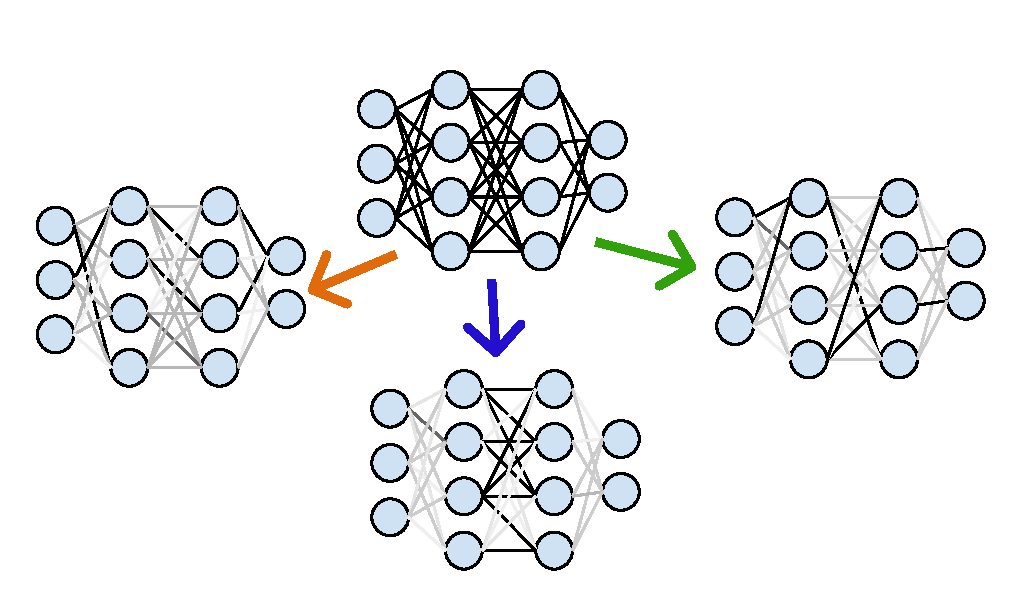
\includegraphics[width=.7\textwidth]{../figures/1b_jacobian_diagram.pdf}
    \end{subfigure}
    \begin{subfigure}{\columnwidth}
        \centering
        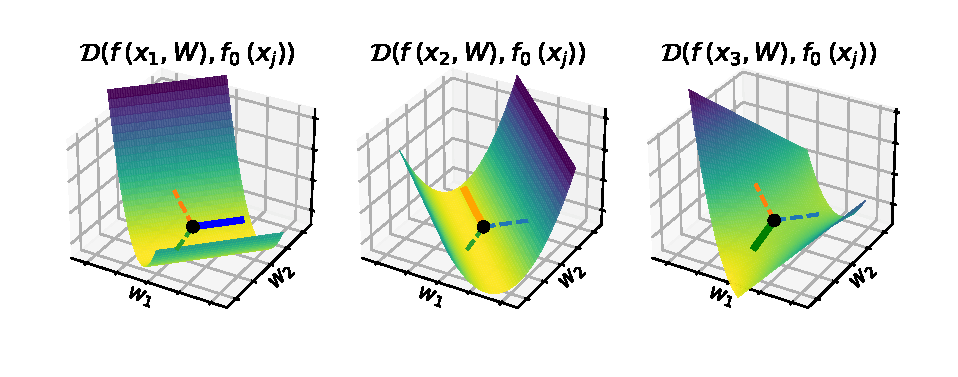
\includegraphics[width=\textwidth]{../figures/1a_jacobian_diagram.pdf}
    \end{subfigure} \caption{Decomposing a loss landscape into a set of parameter directions , where (1) the set of directions can approximately reconstruct any per-sample-pair gradient of divergence and (2) for any given sample, the curvature in most of the subnetworks directions is approximately zero.}\label{fig:1_jacobian_diagram}
    
\end{figure}


Local loss landscape decomposition (L3D) aims to decompose a model's gradients of loss between output pairs with respect to parameter space \ref{fig:1_jacobian_diagram}. We seek to identify directions in parameter space such that (1) the set of directions can approximately reconstruct any gradient of paired sample divergences, and (2) for any given pair of samples, an even smaller subset of directions can be used in reconstructing this gradient. To reduce computational complexity, we learn low-rank representations of these parameter directions. In this work, we first describe the mathematical foundation of our approach. We then develop progressively more complex toy models to measure the efficacy of L3D and quantify its limitations. %Finally, we apply L3D to a real-world model to derive insights into model computation that would not have been possible through activation-based methods. We discuss the strenghts and limitations of L3D, and what we see as future work. 


\section{Methodology}

In the next sections, we will formally setup our decomposition problem (Sec. \ref{sec:setup}), define the criteria we will use for our subnetworks/parameter directions (Sec. \ref{sec:criteria}), describe how to efficiently decompose parameters into these directions (Sec. \ref{sec:decomposition}), walk through our training algorithm (Sec. \ref{sec:training}), and then explain how to use these decompositions to intervene on a model's behavior (Sec. \ref{sec:intervention}). 

The terms parameter directions, subnetworks, and circuits can all be used interchangeably, and will refer to the directions in parameter space that we wish to learn. 

\subsection{Set up}\label{sec:setup}


Consider a model $f$ that takes an batch of inputs $X$ and parameter values of $W$, and outputs a batch of outputs.

\begin{equation}
    f(x, W) : R^{n_s \times n_f} \mapsto R^{n_s \times n_o}
\end{equation}

where $n_s$ is the number of samples in the batch, $n_f$ is the length of each input vector, and $n_o$ is the length of each output vector.

Our project rests on the following hypothesis: 

% Numbered list
\begin{enumerate}
    \item For a given input, there are many components of a model that are not involved in inference. Changing these parameters will not affect change the model's output. 
    \item For the same given input, there are a smaller set of components in a model that are highly involved in inference. Changing these parameters will change the model's output.
    \item We are interested in parameter directions that meaningfully change a model's output. We'd like to identify directions that when perturbed, do not break the model's output by moving it completely outside of realm of realistic outputs, but rather turn decrease or enhance the power of a specific computational circuit. 
\end{enumerate}

\subsection{Divergences of Paired Outputs}\label{sec:criteria}
To put point (3) a different way, intervening in a certain parameter direction should not move our outputs too far away from a reference output distribution. Therefore, we will be decomposing gradients of divergences between pairs of outputs - with the aim of finding directions that move the model's output within the same subspace that the reference output distribution lies. 

Divergence of a pair of outputs can be defined as:
\begin{align}\label{eq:divergence}
    &\nabla_W D(f(x_i, W), f(x_r, W_0))|_{W=W_0} \\
    &\text{ where } x_i, x_r \in X \notag
\end{align}


Here, $D$ is a divergence measuer, $f$ is our model, $x_i$ is our input of interest, $x_r$ is a randomly selected reference input , $W$ is a set of parameters and $W_0$ is model's parameters fixed. Our toy models, which are regression-type models, so we use MSE as divergence.

Wee will abbreviate $f(x_r, W_0)$ as $f(x_r)$ and the expression in Eq. \ref{eq:divergence} as $\nabla_W D$.

\subsection{Sparse Principal Directions}\label{sec:decomposition}

We want to transform our gradient into directions in parameter space, where each sample's gradient can be written as a linear combination of a small set of these components. We will do this by learning transforms $V^{in} \in R^{n_v \times n_w}$ and $V^{out} \in R^{n_w \times n_v}$ where $n_w$ is the number of parameters in the model, and $n_v$ is the number of components (subnetworks) we wish to use to represent the parameter space.

$V^{in}$ effectively transforms a gradient from the parameter space to the subnetwork space, so that: 

\begin{equation}
    \nabla_V D = V^{in} \nabla_W D
\end{equation}

We want to find $V^{in}$ and $V_{out}$ such that for any given pair of samples a small subset of subnetworks can approximately reconstruct the gradient of divergence. 
\begin{align}
    & \nabla_W D \approx {V^{out}}_{:, \mathcal{K}} {V^{in}}_{\mathcal{K},:} \nabla_W D \\
    & \text{ where } \mathcal{K}   = \text{argTopFrac}_k \text{abs}(\nabla_{v_k} D) \notag
\end{align}


$\text{argTopFrac}$ relies on a hyperparameter that controls the number of components we wish to use to reconstruct each sample. In practice, we use a batchTopK \cite{bussmann2024batchtopk} and a fraction rather than an absolute number. If we use a batchTopFrac of .1 it means that we select the top 10\% of $\nabla_V D$ magnitudesover $v_k$ and $x_i$ to reconstruct our batch of gradients.

\subsubsection{Low Rank parameter directions}
Learning a set of full rank parameter parameter directions would be extremely expensive (we would be learning $n_w n_v$ values). We also expect that modular, sparsely active circuits would be lower rank that their full-model counterparts \cite{}. Therefore, we use low-rank representations of our $V^{in}$ and $V^{out}$, and correspondingly learn low-rank circuits. We describe the procedure for doing this in \ref{sec:low_rank}. 


\subsection{Training}\label{sec:training}
We wish to learn the decomposition-related transforms $V^{in}$ and $V^{out}$ that minimize the topK reconstruction loss of our divergence gradient described above. Therefore we use the following L2 norm loss:

\begin{equation}
    L = {|| \nabla_W D - V^{out}_{:,\mathcal{K}} V^{in}_{\mathcal{K},:} \nabla_W D ||}_2
\end{equation}

For each batch of samples, we randomly select a reference sample $x_r$ to be paired with each sample $x_i$ in the batch. We then compute the gradient of divergence of $x_i$ and $x_r$ at the model's current parameters $W_0$. We transform that gradient into the subnetwork space using $V^{in}$, and compute the $\text{topK}$ components. We transform those components back into the original parameter space using $V^{out}$, and compute the loss between the reconstructed gradient and the original gradient. We apply a learning update to $V^{in}$ and $V^{out}$ with the goal of minizing this loss. We also normalize $V^{out}$ to be a unit vector after each update. 


% Algorithm 1
\begin{algorithm}\label{alg:training}
\caption{Training Algorithm}
\begin{algorithmic}[1]
\FOR{each epoch}
    \FOR{each $X$}
        \FOR {each $x_i \in X$}
            \STATE Randomly select $x_r \in X$
            \STATE $\nabla_w D_i = \nabla_w D(f(x_i, W), f(x_r))|_{W=W_0}$
        \ENDFOR
        \STATE $\nabla_v D = {V^{in}} \nabla_w$
        \STATE $\tau = \text{topK}(\text{abs}(\nabla_v D))$
        \STATE $\hat{\nabla}_w D = {V^{out}} (\nabla_v D \odot (\text{abs}(\nabla_v D) > \tau))$
        \STATE $L = {|| \nabla_w D - \hat{\nabla}_w D ||}_2$
        \STATE $L.\text{backward()}$
        \STATE Update $V^{in}$ and $V^{out}$
        \STATE Normalize $V^{out}$ to be unit vectors.
    \ENDFOR
\ENDFOR
\end{algorithmic}
\end{algorithm}

\subsection{Measuring and Intervening}\label{sec:intervention}

Our learned subnetworks will just be the rows of $V^{out}$, reorganized into the same tensor structure as $W$. After identifying subnetworks, we may want to intervene on a specific circuit.

If we wish to intervene using a single subnetwork, we can update the parameters in by moving them in a scalar factor ($\delta$) of that unit direction. To tune our model in the direction of subnetwork $v_i$ and compute predictions on $x$, we evaluate:

\begin{equation}
    f(x, W + \delta v_i)
\end{equation}

Going one step further, we may want to finetune our model, but constrain our finetuning to specific circuits for efficiency or performance reasons. While we do not use finetuning in this work, we describe what the process of finetuning would look like in Appendix \ref{sec:finetuning}.

Additionally, we may want to identify which subnetworks were most relevant to the predictions of various samples, or identify which samples most relied on a given subnetwork. We describe this process in Appendix \ref{sec:impact}


\section{Results}

We designed several toy models to test the efficacy of L3D. Our toy models all consist of several well-characterized computations being performed by the same model, with an input space designed to rely on a single or small set of tasks. By designing our toy models this way, we have well characterized ground truth subnetworks by which to compare L3D's decompositions.

Our toy models progressively test more complex types of circuits. Table \ref{tab:toy_models} describes our 4 toy models and the different attributes of circuitry the are designed to capture. The specific hyperparameters used to train our toy models is described in Appendix \ref{sec:toymodel_hyperparams}, as well as the hyperparmaters used for each decomposition in Appendix \ref{sec:L3D_hyperparams}

\begin{table*}[htb]
    \centering
    \begin{tabularx}{\textwidth}{X X X X X}  % Adjusted for new column structure
        \toprule
         & Toy model of superposition & Circuit Superposition & Higher Rank Circuit Superposition & Complex Loss Landscape \\  
        \midrule

        \hline
        & 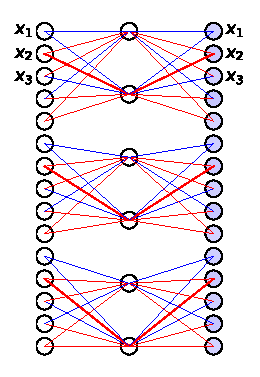
\includegraphics[width=0.12\textwidth]{../figures/2a_toy_models_setup.pdf} &
        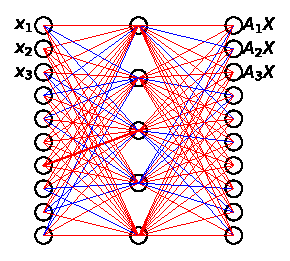
\includegraphics[width=0.2\textwidth]{../figures/2b_toy_models_setup.pdf} &
        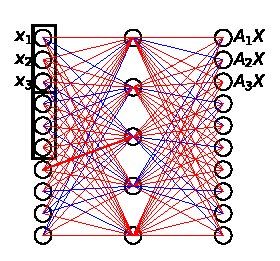
\includegraphics[width=0.2\textwidth]{../figures/2c_toy_models_setup.pdf} &
        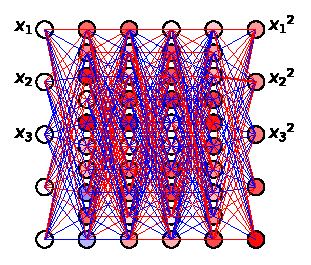
\includegraphics[width=0.2\textwidth]{../figures/2d_toy_models_setup.pdf} \\
         & $X \mapsto X$ & $X \mapsto A X$ & $X \mapsto A X$ & $X \mapsto X^2$ \\  
        Feature Superposition & $\checkmark$ & $\checkmark$ & $\checkmark$ & $\checkmark$ \\  
        Circuit Superposition & $\times$ & $\checkmark$ & $\checkmark$ & $\checkmark$ \\  
        Circuits $>$ rank-2 & $\times$ & $\times$ & $\checkmark$ & probably $\checkmark$ \\  
        Complex Loss Landscape & $\times$ & $\times$ & $\times$ & $\checkmark$ \\  
        \bottomrule
    \end{tabularx}
    \caption{Toy models and their properties (transposed)}
    \label{tab:toy_models}
\end{table*}

\subsection{Toy Model of Superposition}

\subsubsection{Setup}

We start off by validating our algorithm on a well-studied toy problem, the toy model of superposition (TMS), with a small variation. TMS is an autoencoder with a single low-dimensional hidden layer in between and a relu activation at the output \cite{elhage2022toy}. The model is trained on a dataset of samples where few features are active at a time, and "superimposes" these features in the hidden layer such that features embeddings in the hidden layer have minimal interference with each other \ref{fig:s2_tms_encoder_directions}. We train a toy model of superposition with 5 features and 2 hidden dimensions (with 1-sparsity=.05), and then place three such models in parallel, to test our method's ability to resolve superimposed features, as well as indpendent circuit modules.


\subsubsection{Decomposition}
We decompose the TMS model into 15 subnetworks, using rank-1 parameter tensors. The network decomposes into subnetworks as we would expect: each subnetwork represents the embedding and reconstruction of a single input element, involving only the weights connecting the relevant input and output, and the final bias. Fig. \ref{fig:3_tms_subnetworks_first5} shows the subnetworks corresponding to each of the first 5 features, and Fig. \ref{fig:s3_tms_full_subnetworks} shows the full decomposition. One thing to note is that parameter vectors do not have a preferred direction. L3D is equally likely to identify a parameter vector in the direction of $\theta$ as it is in the direction of $-\theta$. This is why, for example, the weights and biases in subnetwork 1 are in the opposite direction as the original network (Table \ref{tab:toy_models}).

This decomposition resulted in a reconstruction error of .19. 15 components of rank-1 can successfully express each individual $X_i:\hat{X}_i$ circuit, but does not capture the interference between features when multiple features are active in the same sample. We expect decompositions of higher dimensional networks to exhhibit less reconstruction error, as the amount of nearly orthogonal parameter vectors (non-interferring) that can be compressed into parameter space scales exponentially with dimension. We see this effect in later toy models. 

%--------------------- FIGURE 2: TMS Subnetworks - First 5 ---------------------
\begin{figure*}
    \centerline{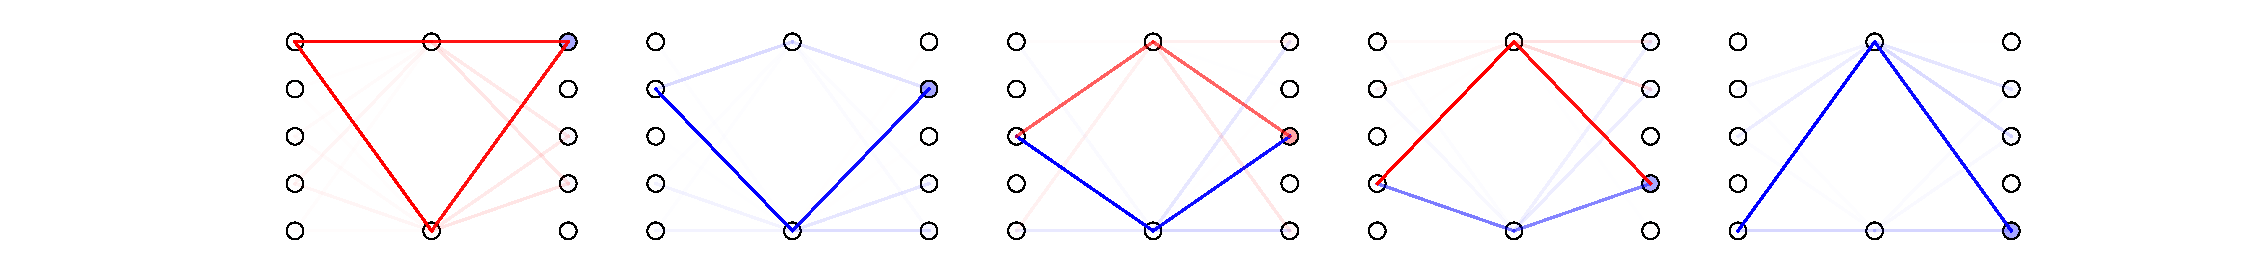
\includegraphics[width=\textwidth]{../figures/3_tms_first_5_subnetworks.pdf}}
    \centering
    \caption{Selected 5 subnetworks that L3D decomposes the TMS-in-parallel model into}\label{fig:3_tms_subnetworks_first5}
\end{figure*}


\subsubsection{Intervention}

Parameter vectors learned by L3D can be used to intervene on model behavior. In principle, we could finetune a model with an adaptor that only changes the parameters of a network in the direction of a specified set of parameter vectors (See Appendix \ref{sec:finetuning}). While we do not go the extent of finetuning a model, we explore the effect of perturbing a model's parameter space in the direction of a subnetwork (by an increment of $\delta$). If subnetworks do in fact represent sparse computations, we hope that intervening on a subnetwork has a strong effect on the predictions of relevant samples, and no effect on other samples. As shown in Fig. \ref{fig:4_tms_intervention}, moving the TMS-in-parallel model in the direction of a single subnetwork does in fact achieve just this. Perturbing in the direction of network 1 primarily affects samples where feature 1 was active, with a small effect on the inputs that had interference to feature 1's embeddings. In fact, for TMS-in-parallel, we can successfully fully "turn off" a computation by moving far enough in the direction of the subnetwork. (Although for models with more complex loss landscapes, turning "off" a computation is not as straightforward, as we will later discuss).

%--------------------- FIGURE 4: TMS Intervention ---------------------
\begin{figure}
    \centerline{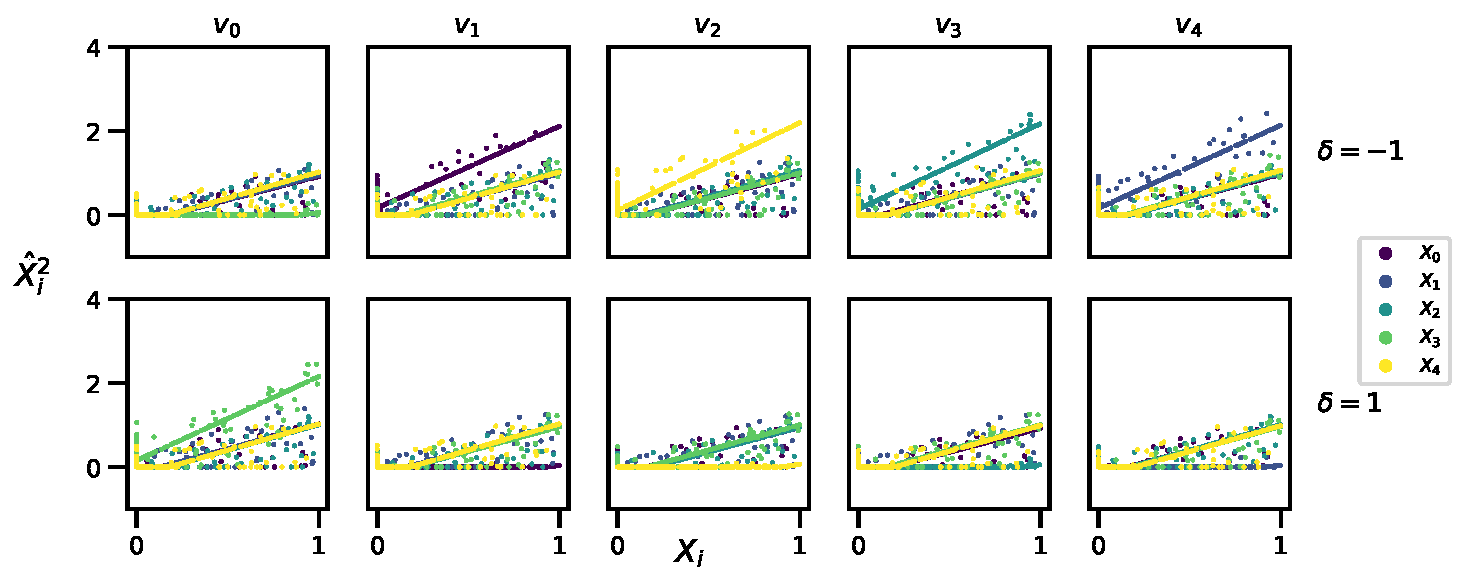
\includegraphics[width=\columnwidth]{../figures/4_tms_intervention.pdf}}
    \centering
    \caption{The effect of intervening on the TMS-in-parallel model in the direction of $\text{Network}_1$.}\label{fig:4_tms_intervention}
\end{figure}

\subsection{Toy Model of Circuit Superposition}

\subsubsection{Setup}


TMS famously exhibits feature superposition - the input elements' low dimenional embeddings are non-orthogonal. However, the sparse circuits in TMS are noteably \textit{not} in superposition - a given weight or parameter is only relevant for a single circuit and circuits. It seems highly unlikely that real world model circuits would decompose this way, since learning circuits composed of non-orthogonal parameter vectors would allow a model to put more expressivitiy into a compressed space. We therefore develop a toy model of \textit{circuit superposition} (TMCS) in order to analyze L3D's ability to resolve such circuits. We define circuit superposition as a phenomenon by which subnetworks share parameter elements, and even more generally have non-orthogonal parameter vectors. 

Our toy model of circuit superposition uses the same architeture and input data distribution as TMS, but is trained to predict linear combinations of the input features as its output ($X \mapsto A X$). We randomly select values of $A$ between 0 and 3 to generate input-output pairs to train the toy model with. We use an input with 10 input features, and 10 output features (although such a model does not need to have the same number of input and outputs).

In this model, if we consider "subnetworks" to be parameter directions involved in inference of a small set of samples, then we would expect each circuit to be associated with a single input feature. If this is the case, then parameters would be involved in multiple circuits: ${W^{dec}}_{i,1}$ (the set of parameters connecting the hidden nodes to the first output node) will contain information about both $A_{1,1}, A_{2,1}, A_{3,1}...$  Put another way, the circuits will interfere with each other - parameter directions associated with each circuit will be non-orthogonal. 

\subsubsection{Decomposition}

We decompose TMCS into 10 subnetworks of rank-1 parameter tensors (\ref{fig:5_circuit_superposition_decomposition}) with a reconstruction loss of .064. The subnetworks look like we expect, with each strongly corresponding to a single input feature.


%--------------------- FIGURE 5: Circuit Superposition ---------------------
\begin{figure*}[htbp]
    \centerline{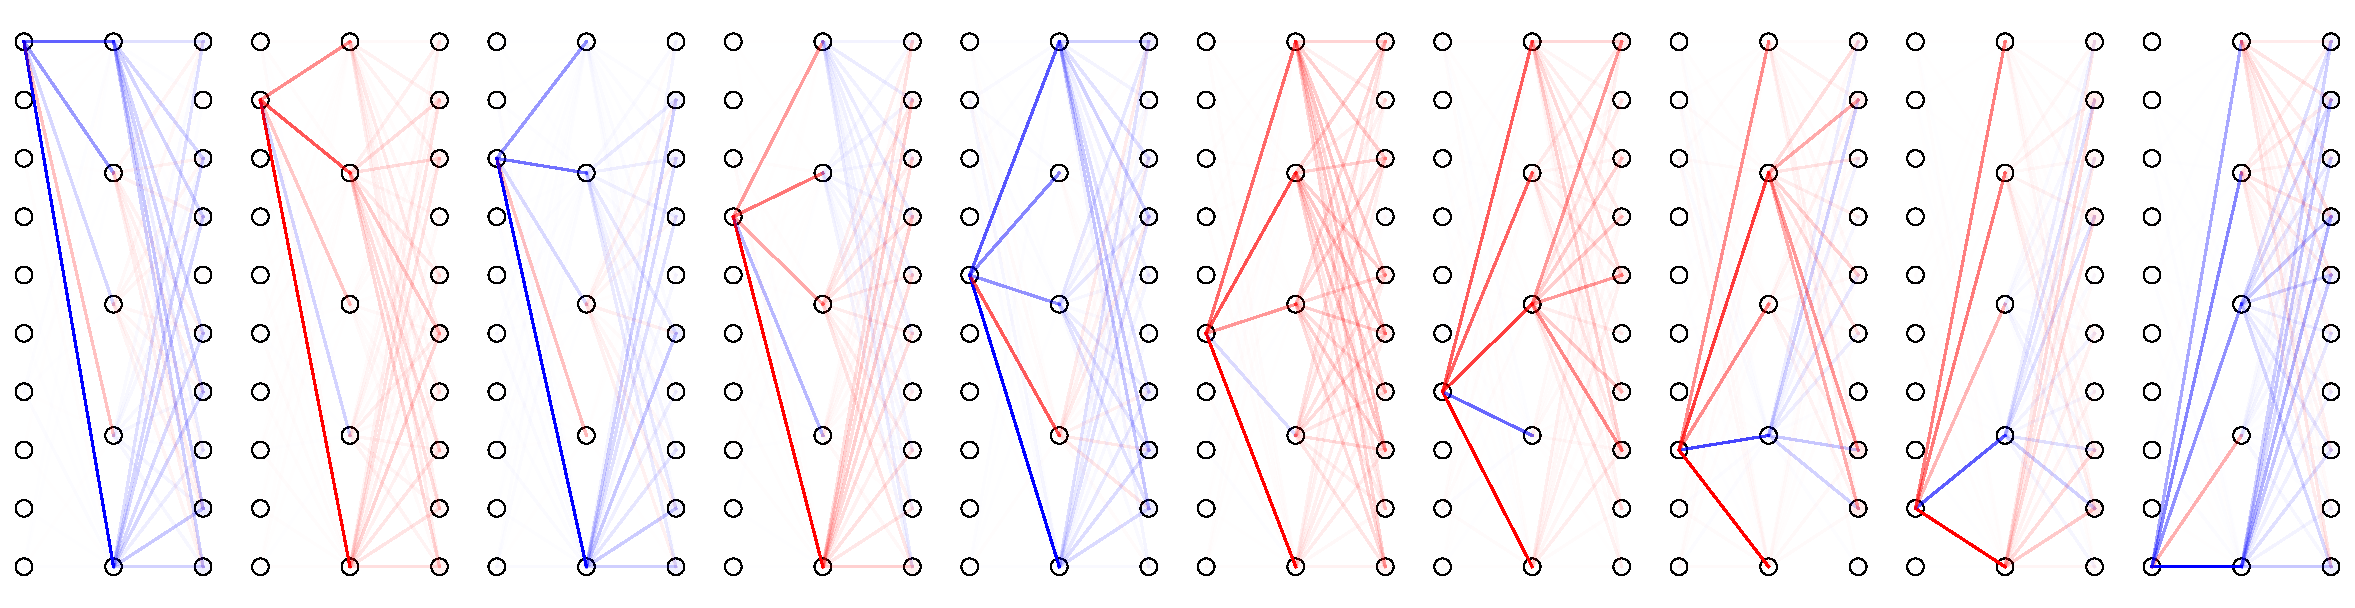
\includegraphics[width=\textwidth]{../figures/5_circuit_superposition_decomposition.pdf}}
    \centering
    \caption{The learned subnetworks of TMCS}\label{fig:5_circuit_superposition_decomposition}
\end{figure*}


Since each subnetwork theoretically corresponds to the computations involved with a single input feature, we should be able to reconstruct the original $A$ values from each subnetwork. To derive $A$ from each subnetwork, we (1) identify the which column in the subnetwork's $W^{dec}$ direction has the largest norm and then (2) trace the weights of the network through that path. That is for subnetwork $k$: 

\begin{align}
    &j^* = argmax_{j} ||{{{W^{dec}}_j}_k}||_2 \\
    &\hat{a}_{i,j} = {{{W^{enc}}_{i,j}}}_k {{W^{dec}}_{i,j}}_k \notag
\end{align}

The parameter vectors are normalized to be unit vectors so we expect them to be a scalar multiple of the true $A$ values. As seen in Figure \ref{fig:5_circuit_superposition_decomposition}, our derived $\hat{\alpha}$ have a very high correlation to the original $A$ values ($r^2 = 0.92$).



%--------------------- FIGURE 6: Circuit Superposition Coefficients ---------------------
\begin{figure}[htbp]
    \centerline{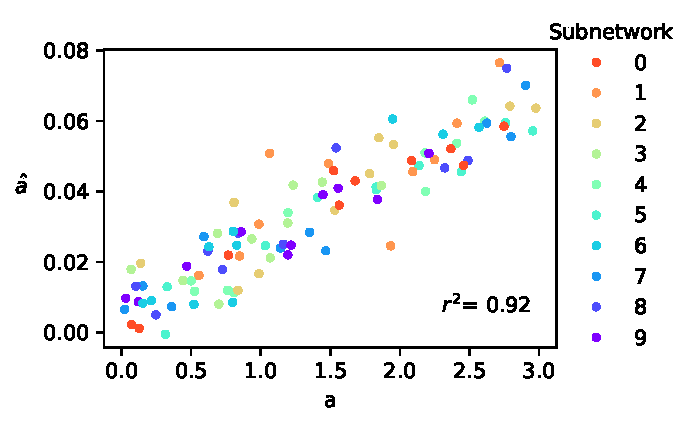
\includegraphics[width=\columnwidth]{../figures/6_circuit_superposition_coefficients.pdf}}
    \centering
    \caption{The coefficients derived from the subnetworks compared to actual coefficients}\label{fig:6_circuit_superposition_coefficients}
\end{figure}


\subsection{Higher Rank Circuits}

\subsubsection{Setup}
Because each subnetwork in TMCS traces the path of a single input neuron, the underlying subnetworks should inherently have a rank of 1. In order to test the ability of L3D to learn higher rank circuits, we developed a toy model with inherently higher rank circuits. For this model, we use the same set up as TMCS, but we correlate the sparsities of sets of input features. We use 25 input features, and we filter our data to ensure that input features 1-5, 6-10, etc, are always active ($>0$) or inactive ($<0$) together. In this setup, circuits should always be associated with groups of 5 input features and so should have a rank of 5.

\subsubsection{Decomposition}

Although we expect the model to have 5 subcircuits, we use excess parameter tensors (n=10) in order to allow more flexibility in learning. We track the fraction of inputs for which a subnetwork was used in the topK reconstruction ($P_{act}$) to identify which were "dead circuits", and report the last epoch. Futhermore, although we expect the underlying subcircuits to be rank 5, we experiment with using different rank representations to see how well lower-rank parameter directions can represent the model. Interestingly, rank-1 representations of the parameter tensors are able to represent the model nearly as well as rank-5 representations (Fig. \ref{fig:s5_high_rank_circuits_loss_vs_rank}). In Fig. \ref{fig:7_high_rank_decomposition}, we show the decomposition of a rank-3 decomposition. L3D successfully learns a subnetwork corresponding to each of the 5 sets of input features, as well as a number of "dead". The higher and lower rank decompositions also learn similar subnetworks (Figure \ref{fig:s6_high_rank_decompositions}). When we trained L3D without these additional subnetworks, the reconstruction loss would get caught in a local minima. Similar to training SAEs \cite{cunningham2023sparse}, having extra degrees of freedom allows for better learning, even if at the end of training the extra subnetworks are never active.


%--------------------- FIGURE 7: Higher Rank Circuit Superposition ---------------------
\begin{figure*}[htbp]
    \centerline{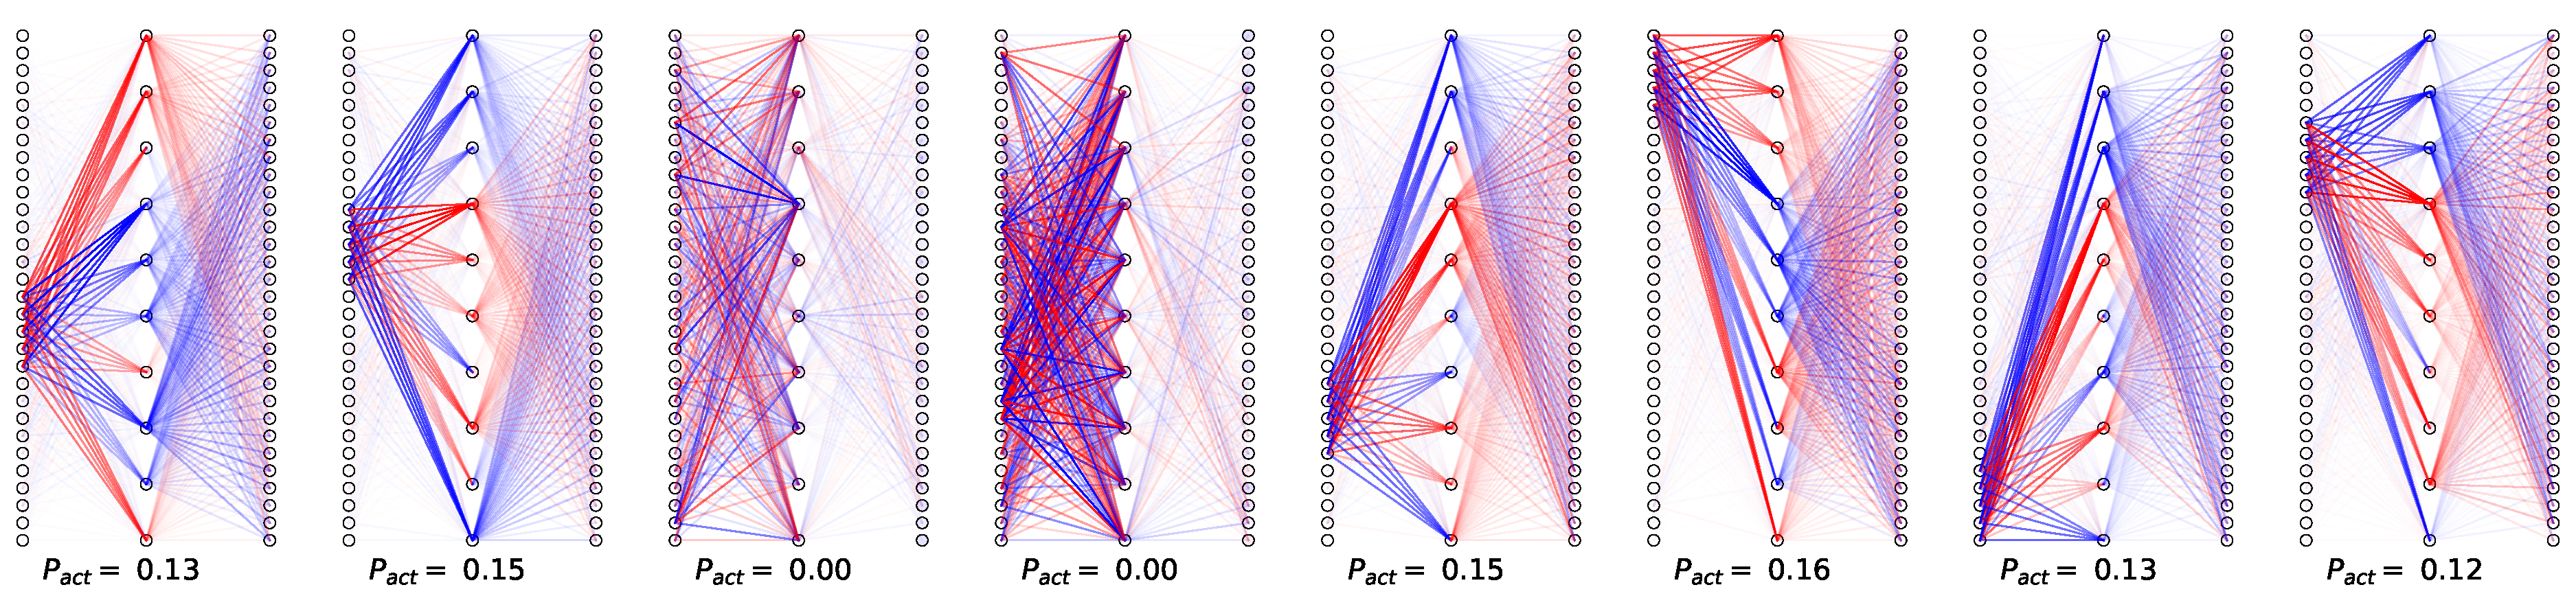
\includegraphics[width=\textwidth]{../figures/7_high_rank_decomposition.pdf}}
    \centering
    \caption{Parameter representations learned by L3D for the high rank circuit decomposition task.}\label{fig:7_high_rank_decomposition}
\end{figure*}


\subsection{Complex Loss Landscape}


\subsubsection{Setup}

The previous set of toy models all had relatively quadratic landscapes with respect to each element of$W^{enc}$ or $W^{dec}$ - $dMSE/dW_i$ depends on $W_i$ to the first order (or not at all, depending on whether the ReLU has fired). This suggests that the local loss landscape of the models is a good approximation for much of the global loss landscape, and we should expect intervening on a circuit to have well-behaved effects, even at large values of $\delta$ (as in Fig. \ref{fig:4_tms_intervention}). 

However, we wanted to test the limitations of a L3D on a model with a more complex loss landscape, especially when it comes to intervening with a subnetwork.

We therefore trained a multi-layer model to predict multiple non-linear functions of input features at once. We train a GeLU network for $X_i \mapsto X_i^2$. We use a network with 4 hidden layers of 5 neurons each, and 5 input and output neurons. Once again, the input features are sparse, incentivizing the toy model to learn circuits in superposition whose interferences will cause minimal errors on the sparse input distribution. 

We expect the model to have 5 subnetworks, one for each input feature. Although it is less clear what rank the tensors of the underlying circuits should be, we expect that with a non-linear model they will likely be high rank. 

\subsubsection{Decomposition}

We decompose our model into 5 rank-2 parameter tensors in our decomposition and instead of varying rank, we experiment with using different numbers of subnetworks to represent our model. In the 5-subnetwork decomposition (Figure \ref{fig:8_squared_subnetworks}), we see that subnetworks tracing the path of $X_i \mapsto X_i^2$ for each input feature $i$. However, this decomposition has a relatively high reconstruction error of .32. Much of this is probably because we kept our topFrac constant throughout all our our models, using a topFrac of .1 for consistency.  With only 5 subnetworks, this means that on average each sample's reconstruction will use <1 subnetwork - limiting the reconstruction error we can achieve. 

We also experiment with holding rank constant (we drop to rank-1) and decompose the model into different numbers of subnetworks (3,5,10, and 15 subnetworks). In our 3-subnetwork decomposition, L3D still learned subnetworks corresponding to single input features, but can of course only represent 3 out of the 5 inputs. As we add more subnetworks, we are able to successfully learn more expressive decompositions of the model that reduce reconstruction error (Figure \ref{fig:s11_squared_features_vs_loss}). Each decomposition continues to learn input-output pair specific subnetworks, with the larger decompositions resulting in a few more dead subnetworks as well (Fig. \ref{fig:s10_squared_decompositions_features}).

%--------------------- FIGURE 8: Squared Model Subnetworks ---------------------
\begin{figure*}[htbp]
    \centerline{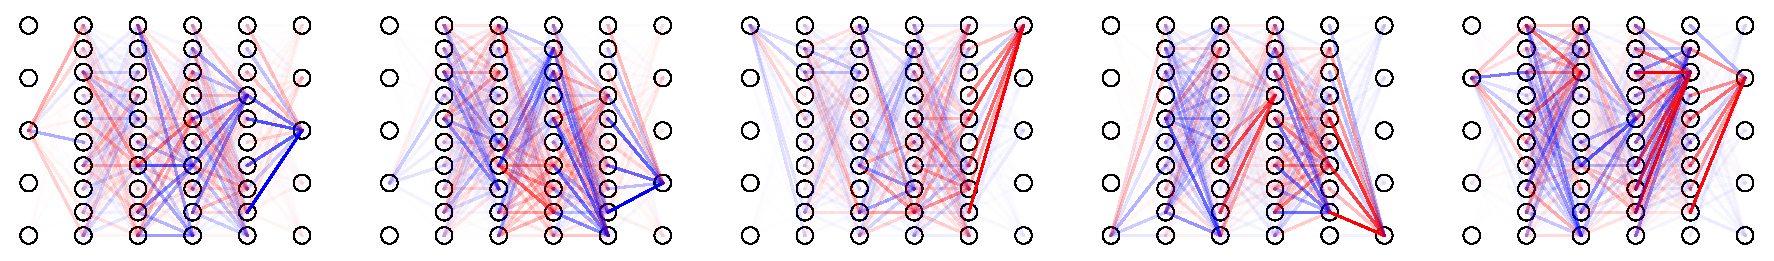
\includegraphics[width=\textwidth]{../figures/8_squared_subnetworks.pdf}}
    \centering
    \caption{Subnetworks learned by L3D for the $X \mapsto X^2$ model, and effect of intervening on each subnetwork}\label{fig:8_squared_subnetworks}
\end{figure*}



\subsubsection{Intervention}

Intervening on these circuits helps us understand how much local loss landscape is representative of global loss landscape, particularly when it comes to inactive subnetworks remaining inactive as we move through parameter space. If local loss landscape is truly representative of global loss landscape in this way, then intervening on on a single subnetwork should result in only a consistent small number of samples being affected, even if we move very far in that direction. Fig. \ref{fig:9_squared_intervention} shows our results for these interventions. Even in this more complex toy model, local loss landscape is a relatively good approximation of the global loss landscape. We can perturb the parameters in a direction of interest and have a large impact on the predictions of that sample and a minor impact on others. If we perturb far enough (Fig. \ref{fig:s7_squared_intervention_more_deltas}), we do begin to see effects on the predictions of other samples, but ratio of change in predictions to the relevant samples to those of the irrelevant samples is very high.



%----------------- FIGURE 9: Squared Subnetworks Intervention ------------------
\begin{figure*}[htbp]
    \centerline{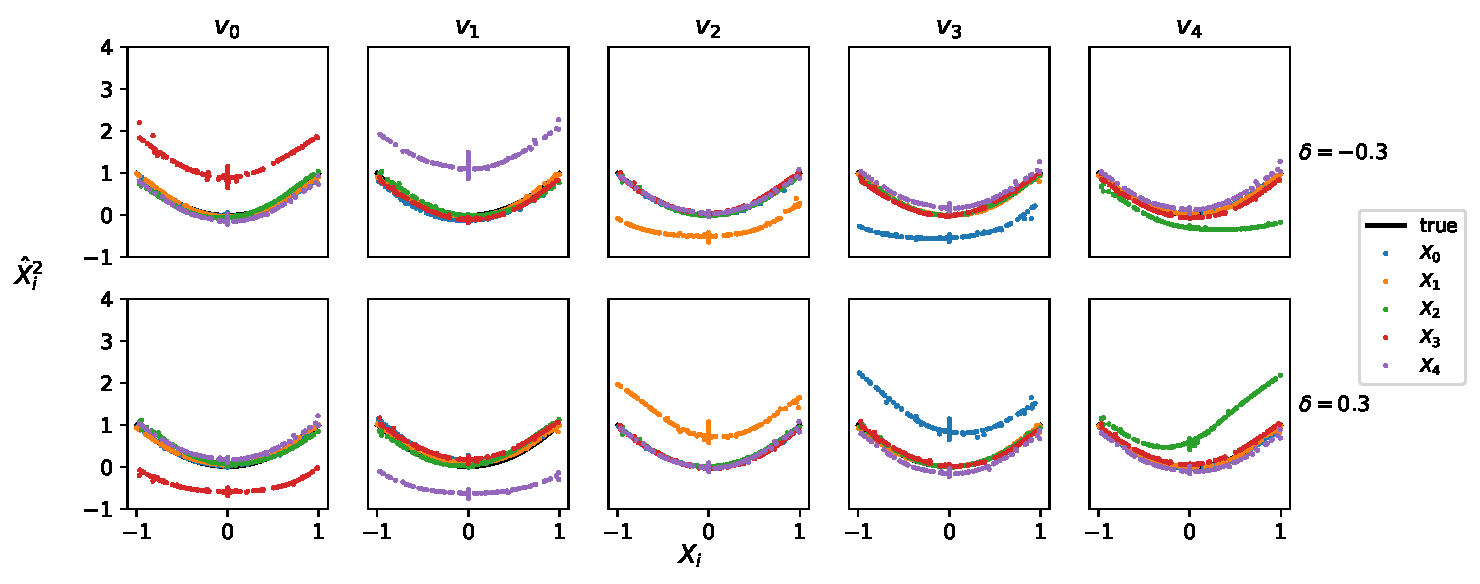
\includegraphics[width=\textwidth]{../figures/9_squared_intervention.pdf}}
    \centering
    \caption{The effect of intervening on each subnetwork}\label{fig:9_squared_intervention}
\end{figure*}


A careful reader may have noticed is that it would be very easy to identify parameter directions in the first or last layer of the $X \mapsto X^2$ model involved in a sparsely active circuit. The circuit for $X_i \mapsto X_i^2$ would just involve all weights connecting input node $i$ to the first hidden layer, and all weights connecting the hidden node $i$ to the output node $i$, as well as the bias of output node $i$. In order to make sure L3D is not just learning this trivial solution, we want to test if the hidden parameter directions it learns are also relevant circuits. Therefore, we perform the same intervention experiments but only interveining with the subnetwork components related to the model's hidden layers' weights and biases (\ref{fig:s8_squared_intervention_middle_weights}). The results are very similar, where inventions on a parameter direction only affect the output of a subset of samples - showing that the circuits that L3D has learned perform relevant computation even in their middle layers. 



\ref{fig:9_squared_intervention} shows changes in predictions as we move in a single direction in parameter space. We also wanted to undrestand how subcircuits might interact with each other as we move through parameter space. In \ref{fig:s9_squared_intervention_multi_features} we perturb multiple subnetworks at once, and measure the new predictions. For the most part, the subnetworks have little inference with each other: the relevant output values for each subnetwork move relatively independently of each other. For some parameter directions, we do see some unexpected interactions, such as when we move in the direction of subnetwork 1 and 2, we see a small effect on the predictions of a few samples not associated with either subnetwork. With larger models, especially those with more modular circuits that are working together, we expect this kind of interaction to become more common. We discuss more in the discussion section. 

\section{Discussion}

\subsection{Simple Improvements}

\textbf{Hyperparameter Choice}

\textbf{Flexible Rank Choices}

\subsection{Challenges}

\textbf{Interpretation of a circuit}

\textbf{Local Loss Landscape}

\textbf{Relationship to overparameterized models}

\subsection{Extensions}

\textbf{Finetuning}

\textbf{Identifying Specific Circuits with Constrastive Pairs}


\clearpage

\section{Impact Statement}

%This paper presents work whose goal is to advance the field of 
%Machine Learning. There are many potential societal consequences 
%of our work, none which we feel must be specifically highlighted here.

% In the unusual situation where you want a paper to appear in the
% references without citing it in the main text, use \nocite

\clearpage
\bibliography{writeup.bib}
\bibliographystyle{icml2025}


%%%%%%%%%%%%%%%%%%%%%%%%%%%%%%%%%%%%%%%%%%%%%%%%%%%%%%%%%%%%%%%%%%%%%%%%%%%%%%%
%%%%%%%%%%%%%%%%%%%%%%%%%%%%%%%%%%%%%%%%%%%%%%%%%%%%%%%%%%%%%%%%%%%%%%%%%%%%%%%
% APPENDIX
%%%%%%%%%%%%%%%%%%%%%%%%%%%%%%%%%%%%%%%%%%%%%%%%%%%%%%%%%%%%%%%%%%%%%%%%%%%%%%%
%%%%%%%%%%%%%%%%%%%%%%%%%%%%%%%%%%%%%%%%%%%%%%%%%%%%%%%%%%%%%%%%%%%%%%%%%%%%%%%
\newpage
\appendix
\renewcommand{\thefigure}{S\arabic{figure}}  % Set figure numbers to S1, S2, etc.
\renewcommand{\theHfigure}{S\arabic{figure}} % Fix hyperlinks in hyperref
\setcounter{figure}{0}  % Reset numbering
\onecolumn


\section{Definitions}

\subsubsection{Dimensions}
$n_s$: The number of samples in a batch of inputs 

$n_f$: The dimensions of a single input vector to a model

$n_o$: The dimensions of a single output vector from a model

$n_w$: The number of parameters values in a model.

$n_v$: The number of subnetworks or parameter directions chosen to decompose a model. 


\subsubsection{Model Syntax}
$X \in \mathbb{R}^{n_s \times n_f}, x \in \mathbb{R}^{n_f}$: Batch and individual input vectors to a model.

$W \in \mathbb{R}^{n_w}, w \in \mathbb{R}$: The set of and individual parameter values of a model

$\mathcal{w}$: The set of parameters corresponding to a specific tensor or block in a model.

$f: \mathbb{R}^{n_s \times n_f} \mapsto \mathbb{R}^{n_s \times n_o}$: A model mapping a set of input vectors to a set of output vectors.

$f(X, W)$: The output of model $f$ with parameter values $W$ on input $X$.

$f(X, W_0)$ or $f(X)$: The output of model $f$ with fixed parameter values $W_0 $. $W_0$ is the set of learned parameter values from model training.

$D$: Divergence metric between two vectors. Typical divergence metrics are mean-squared error for regression-type outputs, and KL-divergence for probability-type outputs. 

\subsubsection{Decomposition Syntax}
$V (or V^{out}) \in \mathbb{R}^{n_v \times n_w}, v (or V^{out})  \in \mathbb{R}^{n_w}$: The set of or individual parameter directions that are used to decompose a model. $V_out$ can be used to transform parameter directions in the subnetwork vector space back into the original parameter space of the model. The terms parameter direction, subnetwork, and circuit all have the same meaning. 

$\mathcal{V}_{out}, \mathcal{v}_{out}$: Components of $V^{out}$ or $V^{out}$ related to a specific tensor or block in the original model. 

$V^{in} \in \mathbb{R}^{n_w}, V^{in} \in \mathbb{R}$: Transforms the original parameter space of the model into the subnetwork vector space. 

$\mathcal{V}_{in}, \mathcal{v}_{in}$: Components of $V^{in}$ or $V^{in}$ related to a specific tensor or block in the original model. 

$r$: The rank of each component of the decomposition vectors corresponding to tensors in the original model. 

\subsubsection{Training}

$\mathcal{K}$: The subset of indexes >= $\tau$ where $\tau$ is the threshold computed by using the top $k$ absolute values in a tensor. 

$L$: The L2 reconstruction loss used to optimize $V^{in}$ and $V^{out}$.

\subsubsection{Measuring and Intervention}
$I(x_i, x_j, v_k), I(x_i, v_k)$: The impact of subnetwork $v_k$ on the divergence between samples $x_i$ and $x_j$, or averaged across many $x_j$ reference samples.

$\delta$: A scalar value to move $W$ in a specific direction. 


\section{Additional Methods}

\subsection{Low-Rank Tensor Representation}\label{sec:low_rank}

We use low-rank representations of our $V^{in}$ and $V^{out}$, and correspondingly learn low-rank circuits.

While $W$ is a vector of all of the parameters in a model, typically model parameters are organized into tensors $W=\{w_i\}_i$. 

If our parameters are organized into tensors $W=\{w_i\}_i$, each subnetwork or parameter component can be organized as $V^{in}_i  = {\{{v^{in}}_i\}}_i, V^{out}_i = {\{{v^{out}}_i\}}_i$ where we have parts of our subnetworks corresponding to each tensor in the original model parameters. We wish each of these tensors to be low rank, and we express them using the canonical polyadic decomposition \cite{} (a way to write 3+ dimentinoal tensors in terms of low-rank components).

\begin{equation}
{v^{in}}_{i,j} = \sum_{r=1}^{R} a_{i,j,r} \times b_{i,j,r} \times c_{i,j,r} ...
\end{equation}

Where $R$ is the rank we wish to use to represent the parameter component, and the number of factors (a, b, c,...) in the factorization is equal to the number of dimensions in the tensor $w_i$.

\subsection{Finetuning}\label{sec:finetuning}

To finetune a model on a specific set of parameter directions, we would freeze the current set of weights and learn an adaptor consisting of linear combinations of the subnetworks of choice. During fine tuning, we would only need to learn the coefficients of these linear combinations greatly reducing cost.

\begin{equation}
    f(X, W_0 + W_{ft} V^{out}_\mathcal{K})
\end{equation}

\subsubsection{Quantifying Impact}\label{sec:impact}

We can quantify the impact of a subnetwork in two ways. First, we can compute the impact of a subnetwork on a pair of samples $x_i, x_j$, identyfing the subnetwork that, if intervened upon, would most strongly impact the the divergence of $x_i$'s outputs when compared to $x_j$. The impact of subnetwork $v_k$ on such a pair of samples, $I(x_i, x_j, v_k)$ can be measured by:

\begin{equation}
    I(x_i, x_j, v_k) = \\
    \left| V^{in}_{k,:} \nabla_w D(f(x_i, W), f(x_j)) \right|
\end{equation}

Alternatively, we can average the impacts of a subnetwork $v_k$ and an input $x_i$ over many different reference samples to better quantify the impact of the subnetwork on a single sample's predictions overall. Although more computationally expensive, this can give a more robust measurement for the impact of a subnetwork on a specific sample. 

\begin{equation}
    I(x_i, v_k) = \frac{1}{n_j} \sum_{j=1}^{n_j} I(x_i, x_j, v_k)
\end{equation}


\subsection{Toy Model Training}\label{sec:toymodel_hyperparams}

For all of our toy models (except the $X \mapsto X^2$ model), we generate uniformly random inputs between 0 and 1. For $X \mapsto X^2$, we generate uniformly random inputs between -1 and 1. For all toy model data, we use a sparsity value of 1-sparsity=.05. We generate 10000 datapoints and train for 1000 epochs with batch sizes of 32. We use an AdamW optimizer with a learning rate of 0.001. 

\subsection{L3D Model Training}\label{sec:L3D_hyperparams}

To train L3D, we use the same training distributions as in each toy models. Although optimal hyperparameter values probably depend on the model size, and the rank and number of parameter tensors, we use the same hyperparameters for all of our models. We generate only 1000 datapoints, with a batch size of 32, and train for 1000 epochs. We use an AdamW optimizer with a learning rate of 0.01, and a learning decay rate of .8 every 100 steps. We always use a topFrac value of .1.  We include all of the model's parameter tensors, including biases, in the decomposition. 

\section{Supplemental Figures}


% ---------------------Figure S1 TMS subnetwork decomposition-------------------------
\begin{figure}[ht]
    \centerline{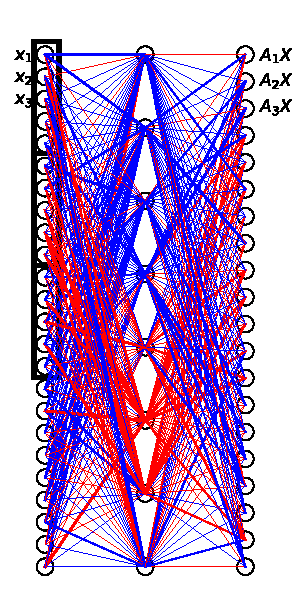
\includegraphics{../figures/s1_high_rank_circuit_setup.pdf}}
    \centering
    \caption{Full architecture of high rank circuit toy model.}\label{fig:s1_high_rank_circuit_setup}
\end{figure}



% ---------------------Figure S2 TMS subnetwork decomposition-------------------------
\begin{figure}[ht]
    \centerline{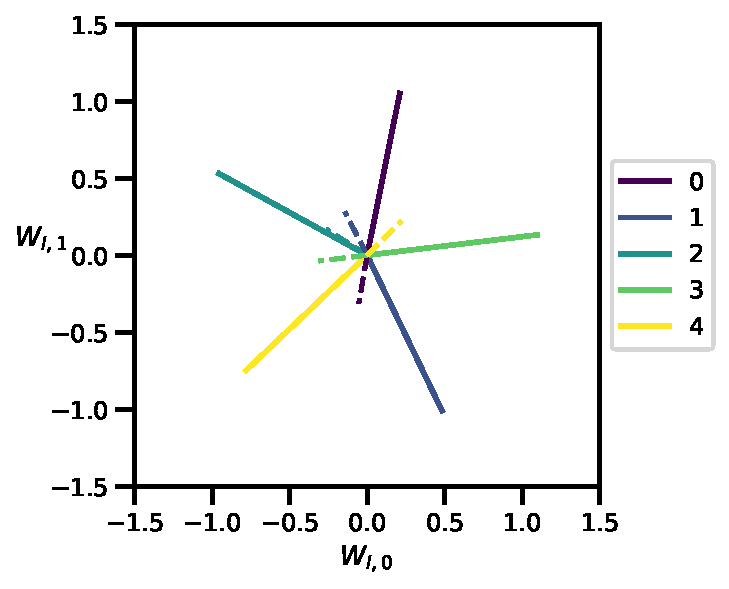
\includegraphics{../figures/s2_tms_encoder_directions.pdf}}
    \centering
    \caption{Encoder directions in TMS}\label{fig:s2_tms_encoder_directions}
\end{figure}


% ---------------------Figure S2 TMS subnetwork decomposition-------------------------
\begin{figure}[ht]
    \centerline{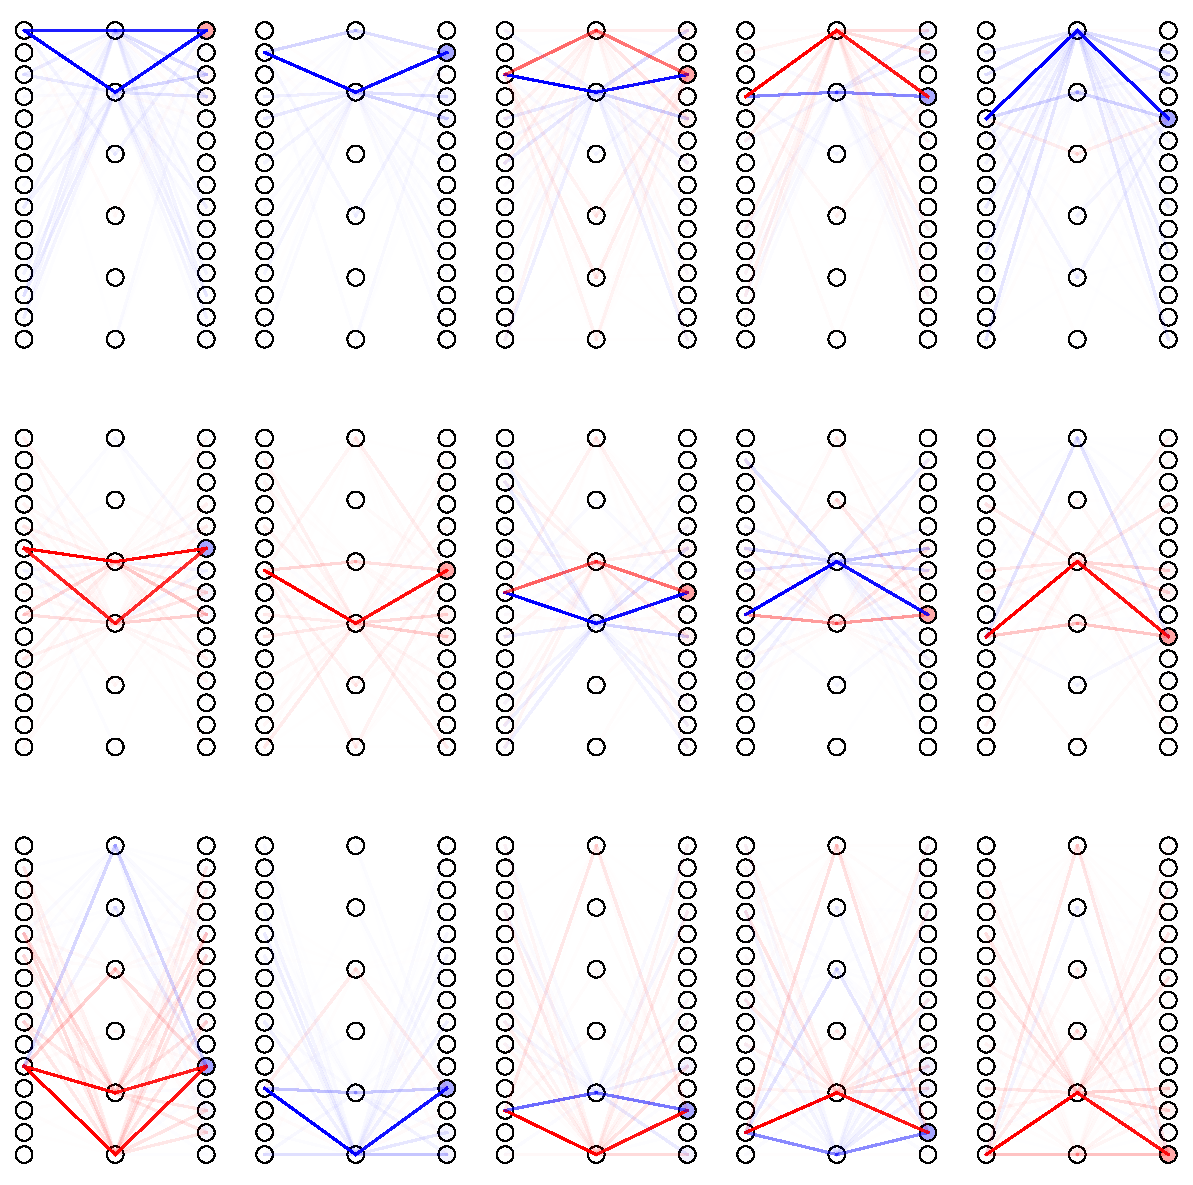
\includegraphics[width=\textwidth]{../figures/s3_tms_full_subnetworks.pdf}}
    \centering
    \caption{All subnetworks for the TMS decomposition}\label{fig:s3_tms_full_subnetworks}
\end{figure}


% ---------------------Figure S3: Intervention on TMS-in-parallel-------------------------
\begin{figure}[ht]
    \centering
    \caption{Effect of intervening on the first 5 subnetworks of the TMS-in-parallel model.}
    \label{fig:s3_tms_interventions}

    \begin{minipage}{\textwidth} % Ensure figures align
        \centering
        \begin{tabular}{cc}  % 3 columns
            \begin{subfigure}{0.3\textwidth}
                \centering
                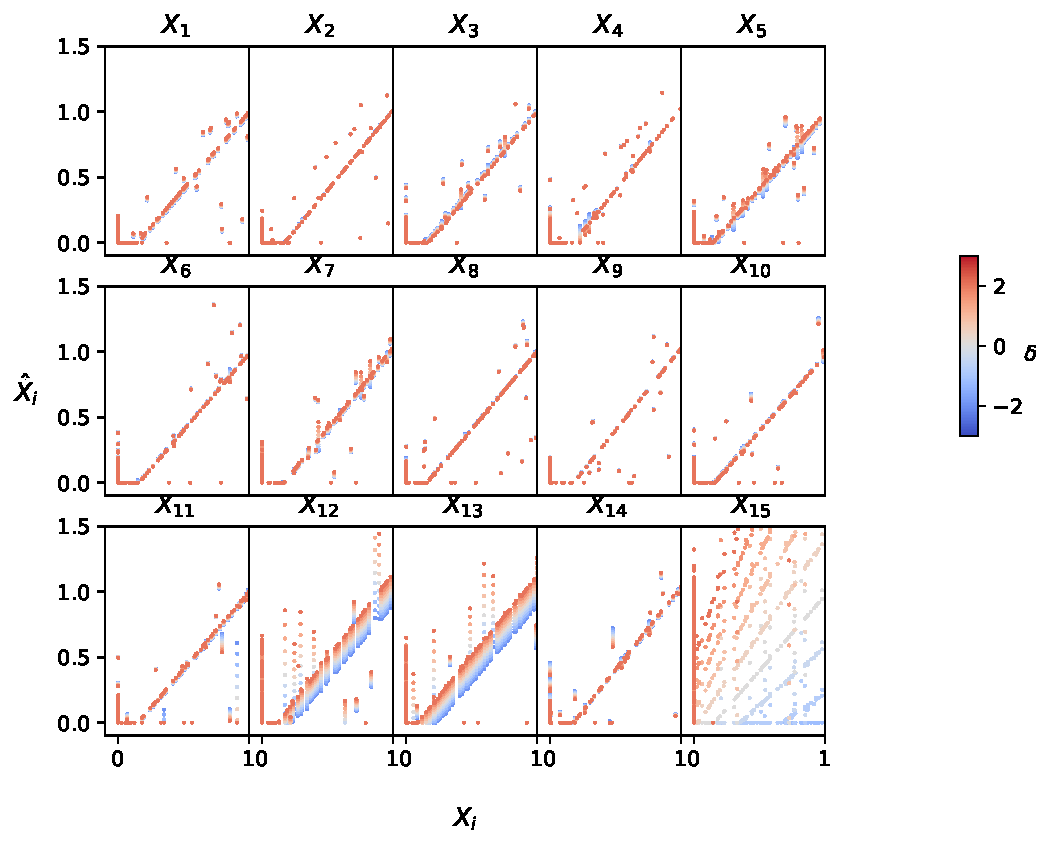
\includegraphics[width=\linewidth]{../figures/s4_tms_intervention_network1.pdf}
                \caption{Subnetwork 1}
            \end{subfigure} &
            \begin{subfigure}{0.3\textwidth}
                \centering
                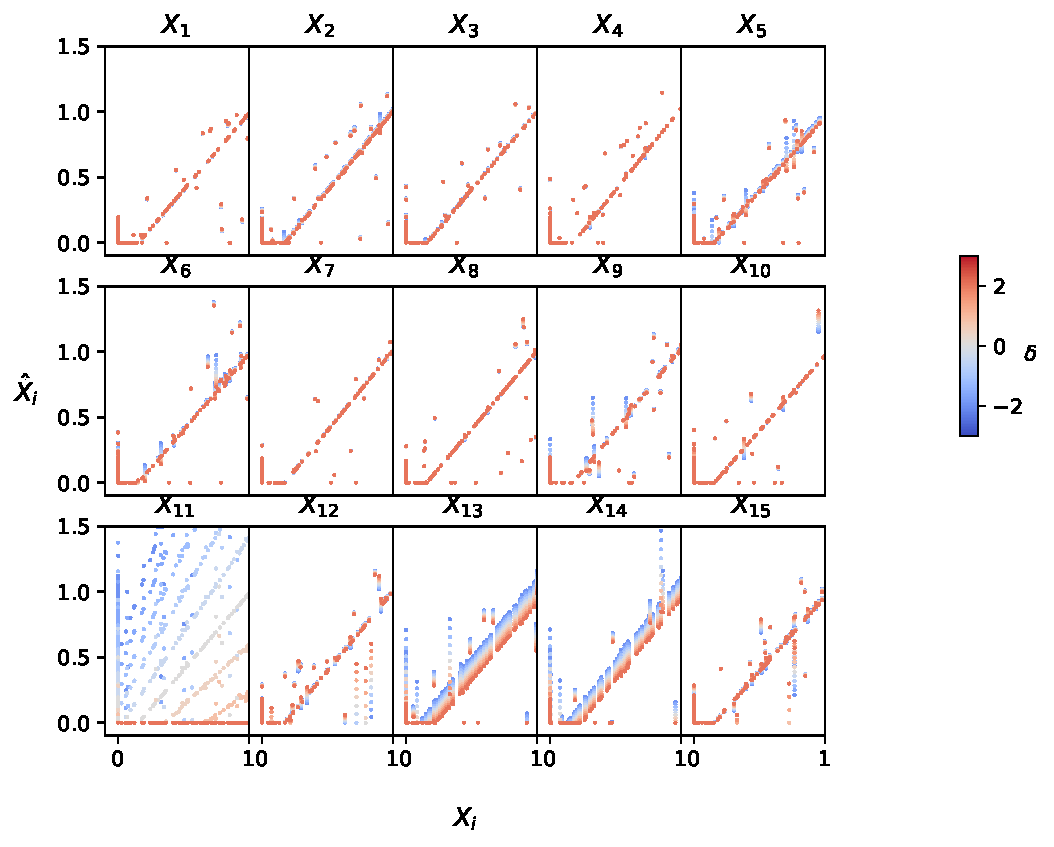
\includegraphics[width=\linewidth]{../figures/s4_tms_intervention_network2.pdf}
                \caption{Subnetwork 2}
            \end{subfigure} \\ % Move to the next row
            \begin{subfigure}{0.3\textwidth}
                \centering
                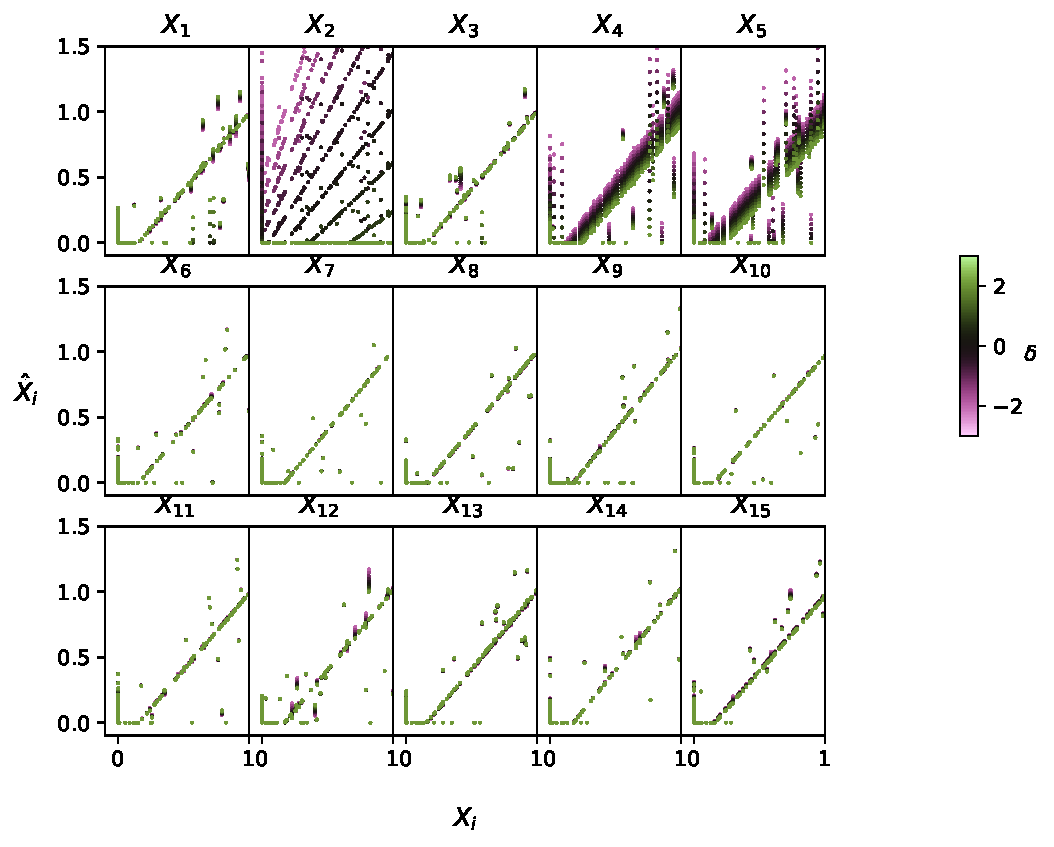
\includegraphics[width=\linewidth]{../figures/s4_tms_intervention_network3.pdf}
                \caption{Subnetwork 3}
            \end{subfigure} & % Move to the next row
            
            \begin{subfigure}{0.3\textwidth}
                \centering
                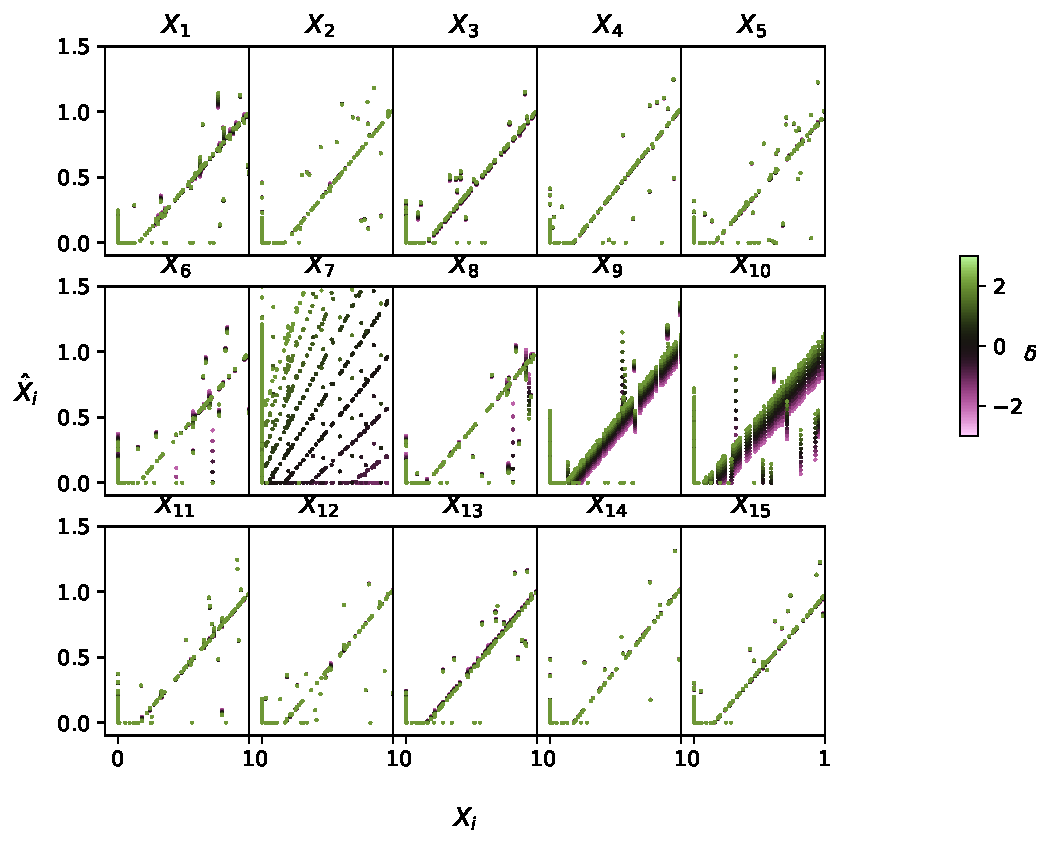
\includegraphics[width=\linewidth]{../figures/s4_tms_intervention_network4.pdf}
                \caption{Subnetwork 4}
            \end{subfigure} \\
            \hspace{\fill} % Spacer to align
            \begin{subfigure}{0.3\textwidth}
                \centering
                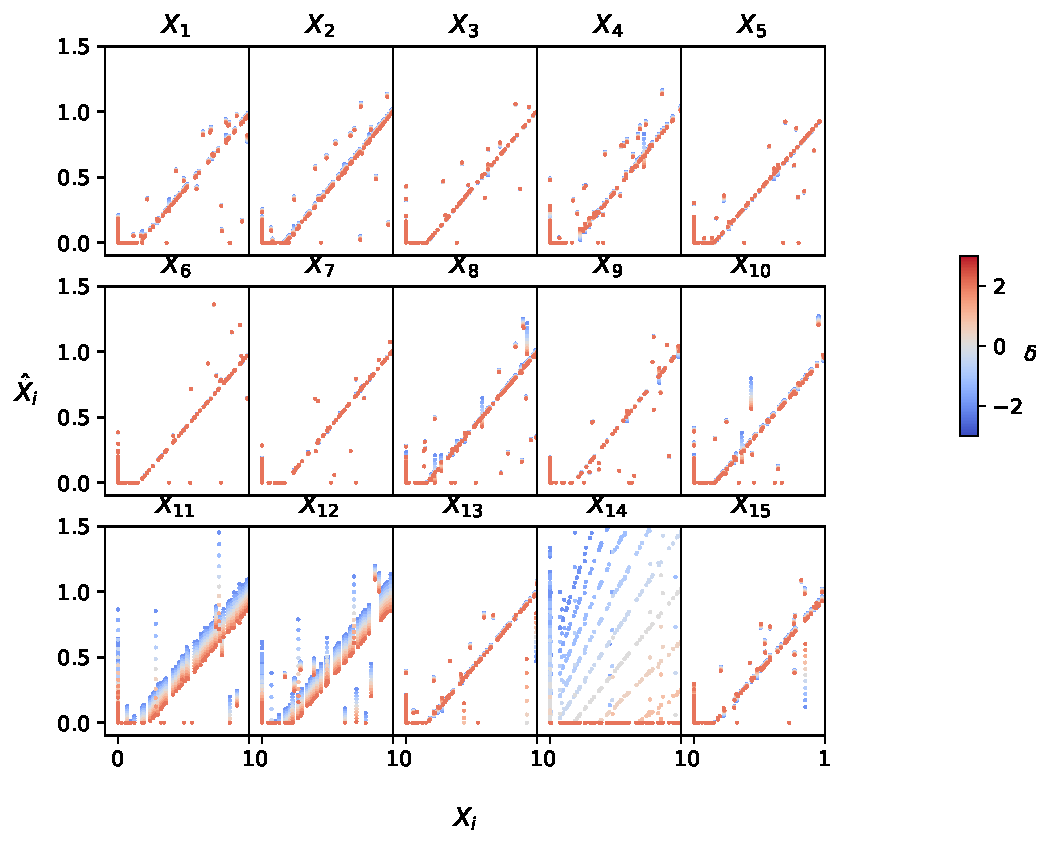
\includegraphics[width=\linewidth]{../figures/s4_tms_intervention_network5.pdf}
                \caption{Subnetwork 5}
            \end{subfigure} &
            \hspace{\fill} % Spacer to align
        \end{tabular}
    \end{minipage}

\end{figure}


%---------------- FIGURE S6: Higher Rank Circuit Superposition ----------------
\begin{figure}[ht]
    \centerline{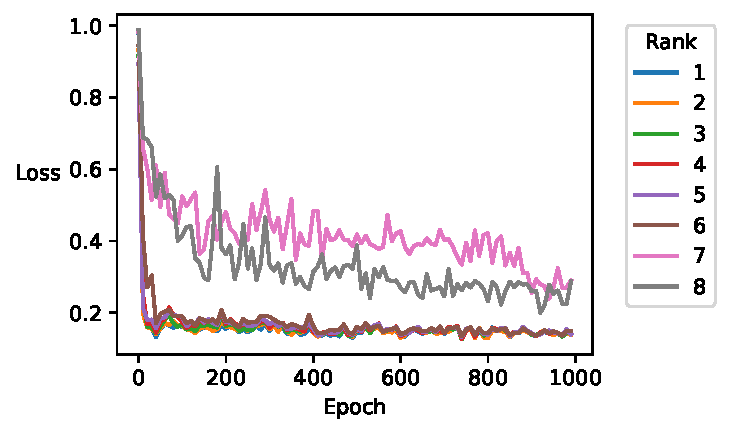
\includegraphics{../figures/s5_high_rank_circuits_loss_vs_rank.pdf}}
    \centering
    \caption{Loss vs Rank}\label{fig:s5_high_rank_circuits_loss_vs_rank}
\end{figure}

  
\begin{figure}[ht]
    \centering
    \caption{Decomposing the toy model of high rank circuits into different numbers of subnetworks}\label{fig:s6_high_rank_decompositions}
    \begin{minipage}{\textwidth} % Ensure figures align
        \centering
        \begin{tabular}{c}  % 3 columns
            \begin{subfigure}{0.3\textwidth}
                \centering
                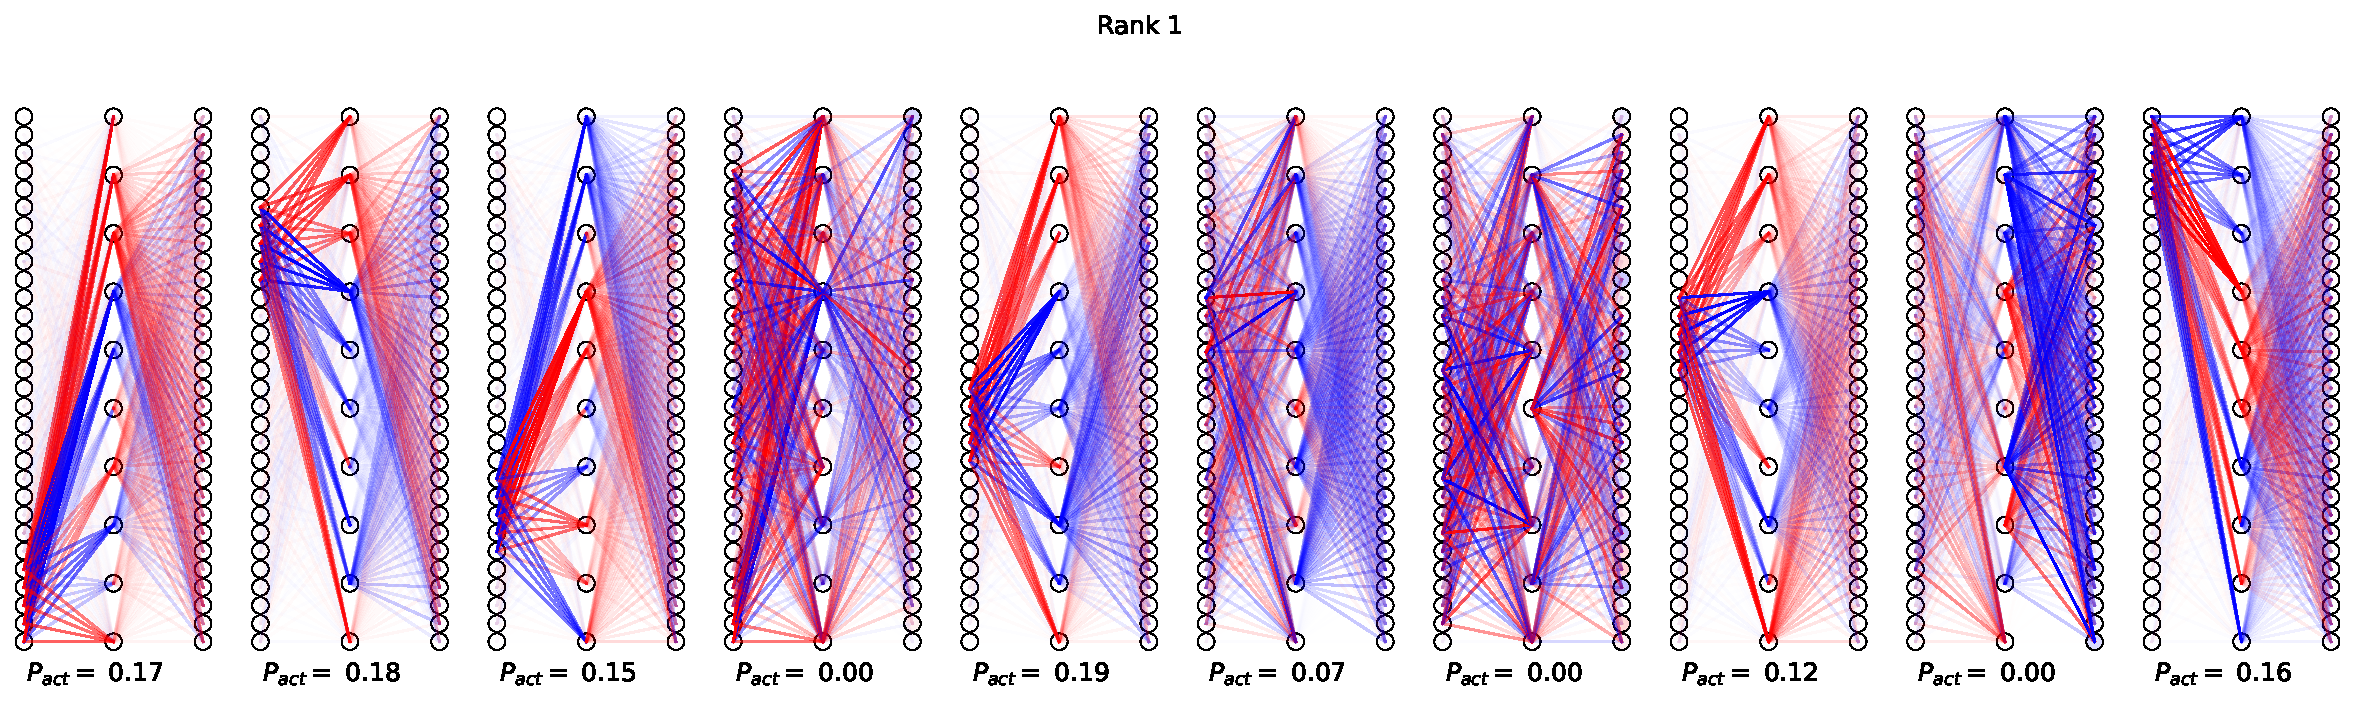
\includegraphics[width=\linewidth]{../figures/s6_high_rank_decompositions_rank1.pdf}
                \caption{Rank-1 Networks}
            \end{subfigure} \\
            \begin{subfigure}{0.3\textwidth}
                \centering
                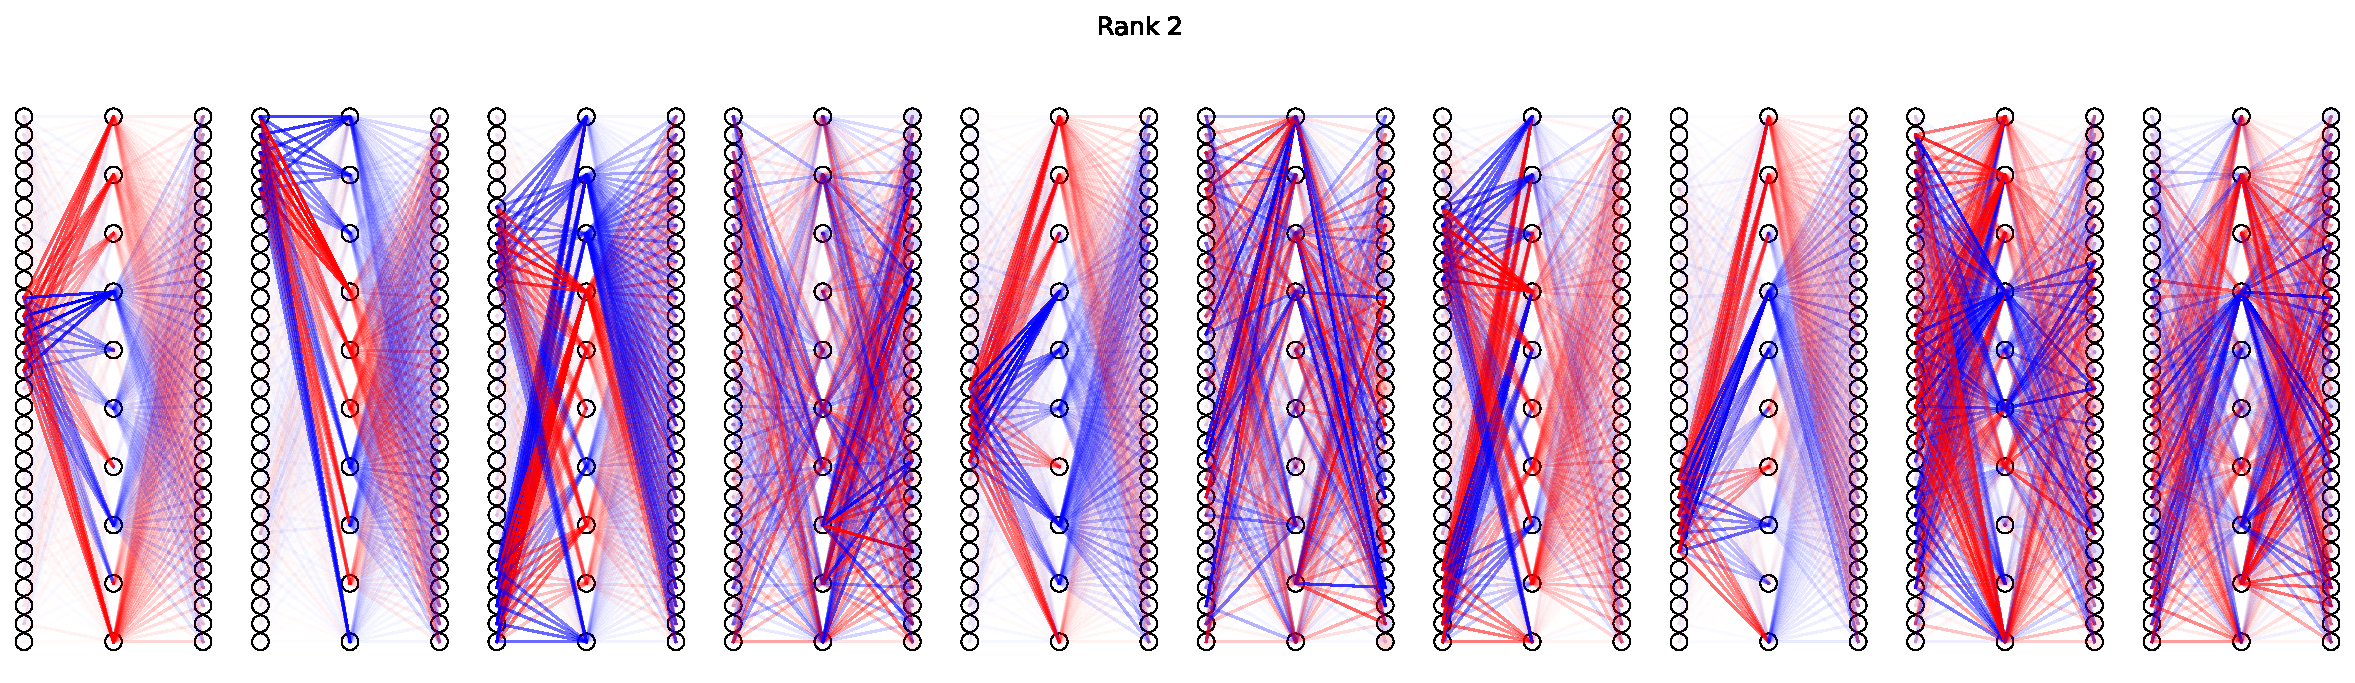
\includegraphics[width=\linewidth]{../figures/s6_high_rank_decompositions_rank2.pdf}
                \caption{Rank-2 Networks}
            \end{subfigure} \\
            \begin{subfigure}{0.3\textwidth}
                \centering
                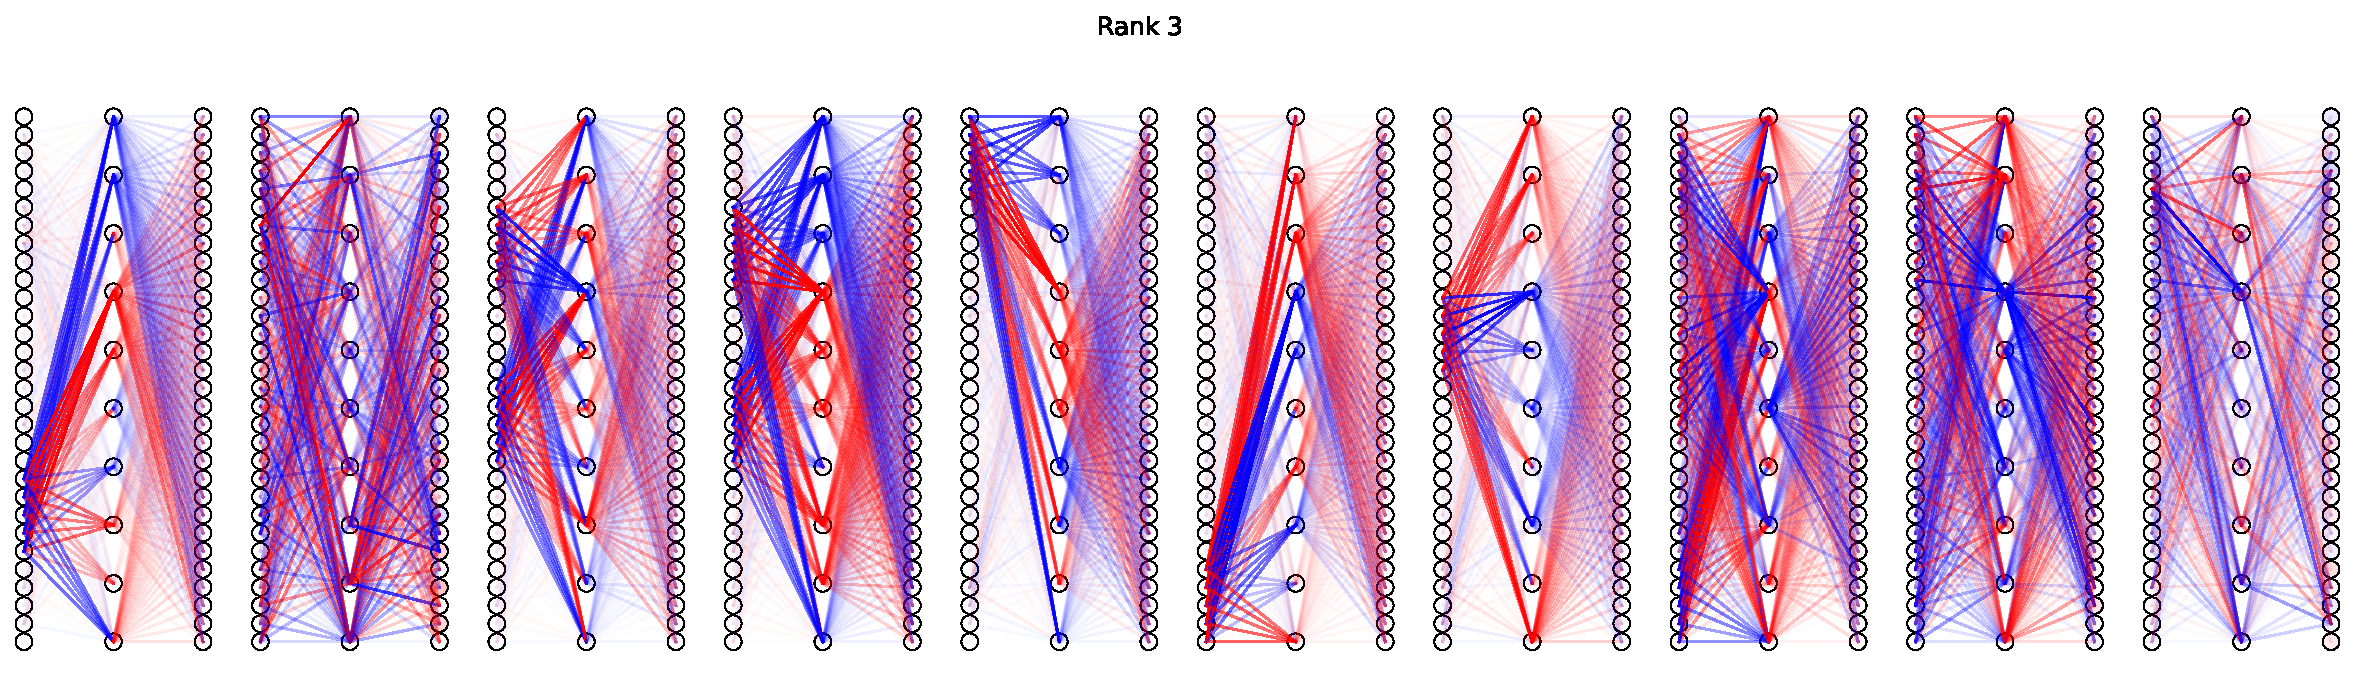
\includegraphics[width=\linewidth]{../figures/s6_high_rank_decompositions_rank3.pdf}
                \caption{Rank-3 Networks}
            \end{subfigure} \\
            \begin{subfigure}{0.3\textwidth}
                \centering
                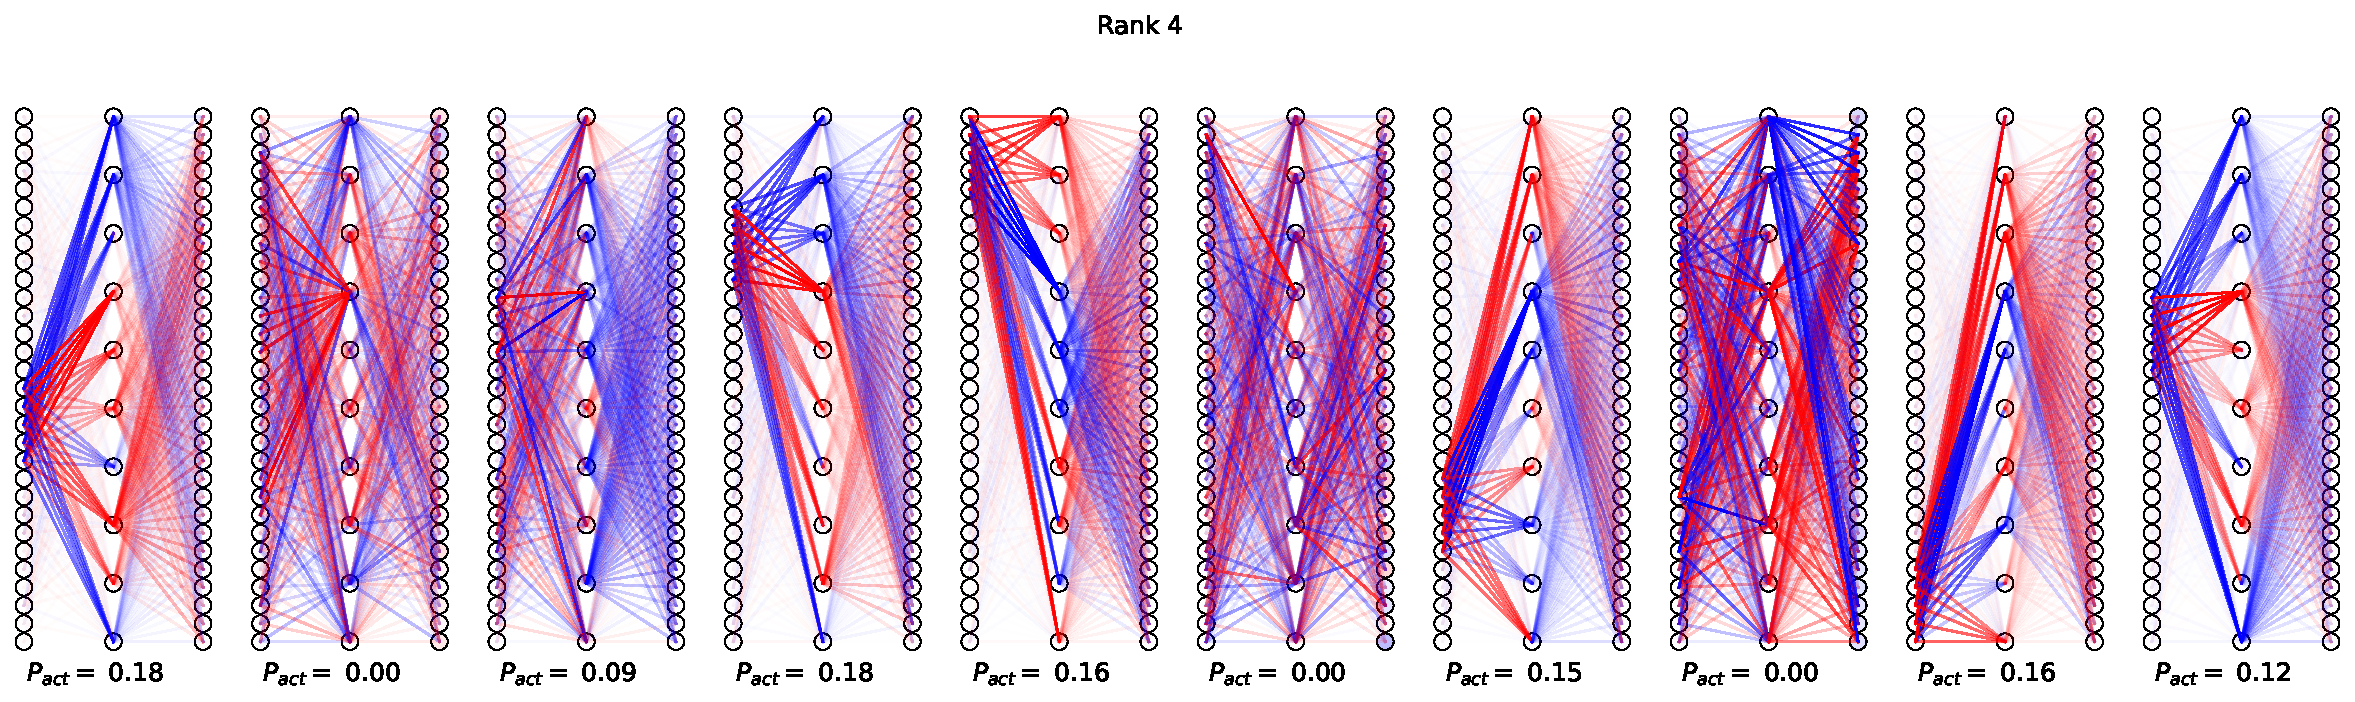
\includegraphics[width=\linewidth]{../figures/s6_high_rank_decompositions_rank4.pdf}
                \caption{Rank-4 Networks}
            \end{subfigure} \\
            \begin{subfigure}{0.3\textwidth}
                \centering
                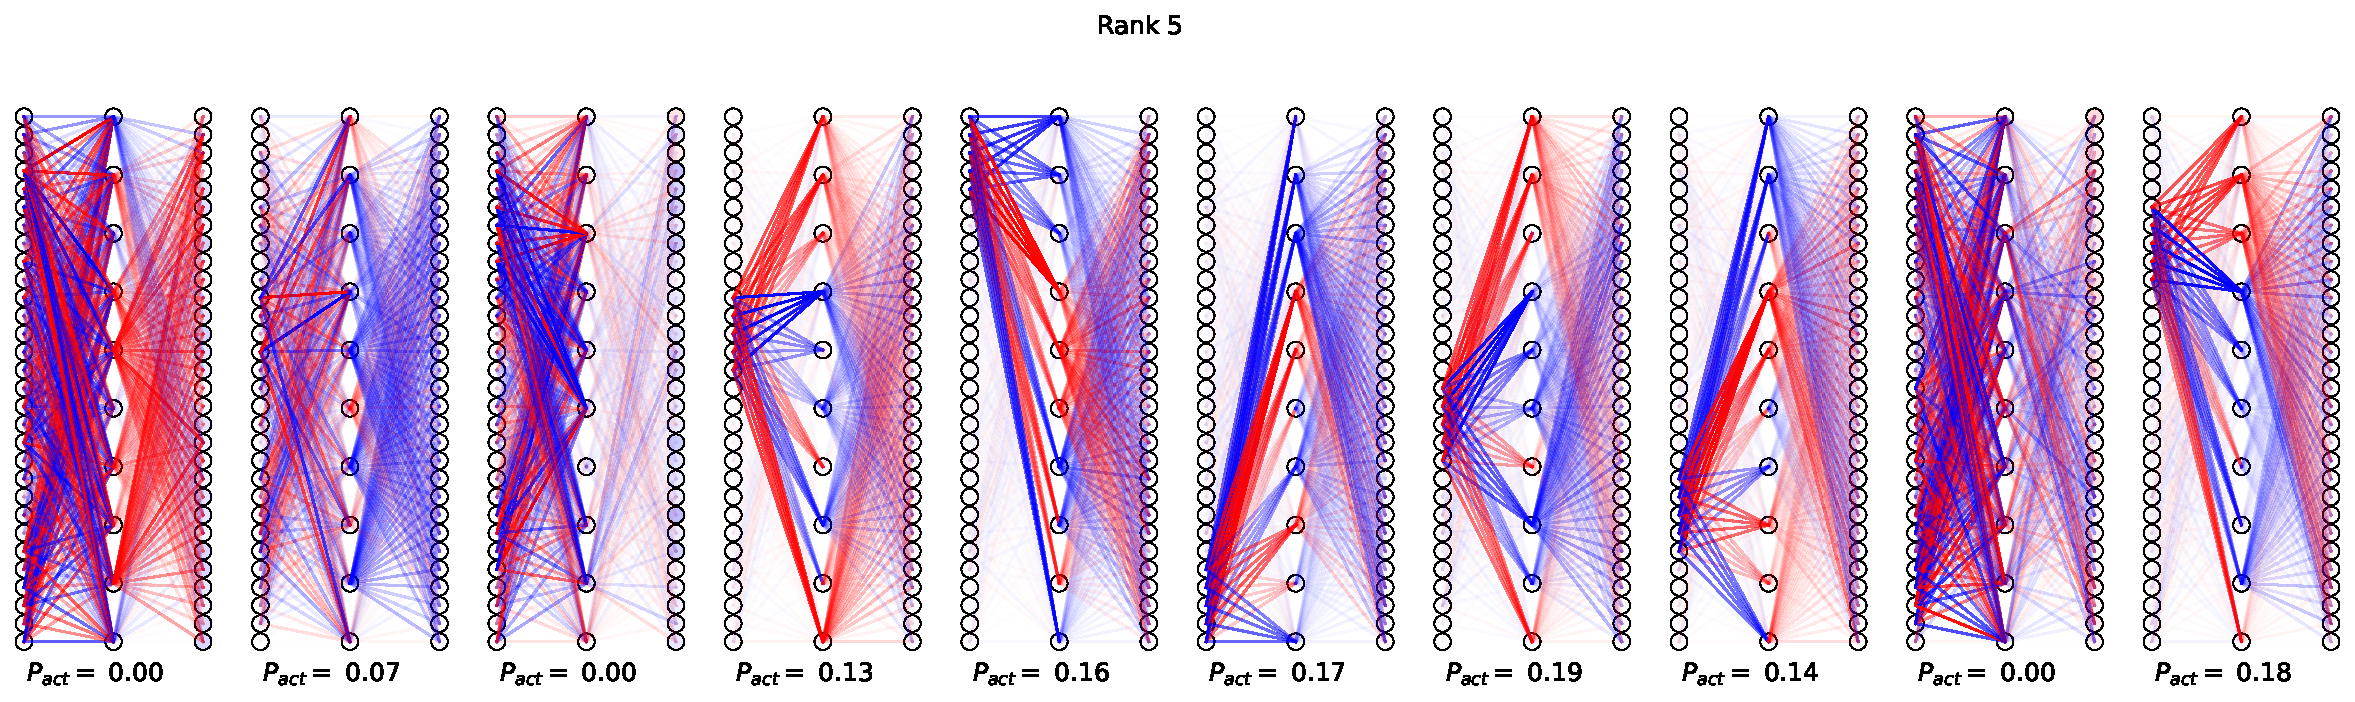
\includegraphics[width=\linewidth]{../figures/s6_high_rank_decompositions_rank5.pdf}
                \caption{Rank-5 Networks}
            \end{subfigure}  
        \end{tabular}
    \end{minipage}

\end{figure}

%--------------------- FIGURE S7: Squared Model More Deltas---------------------
\begin{figure}[ht]
    \centerline{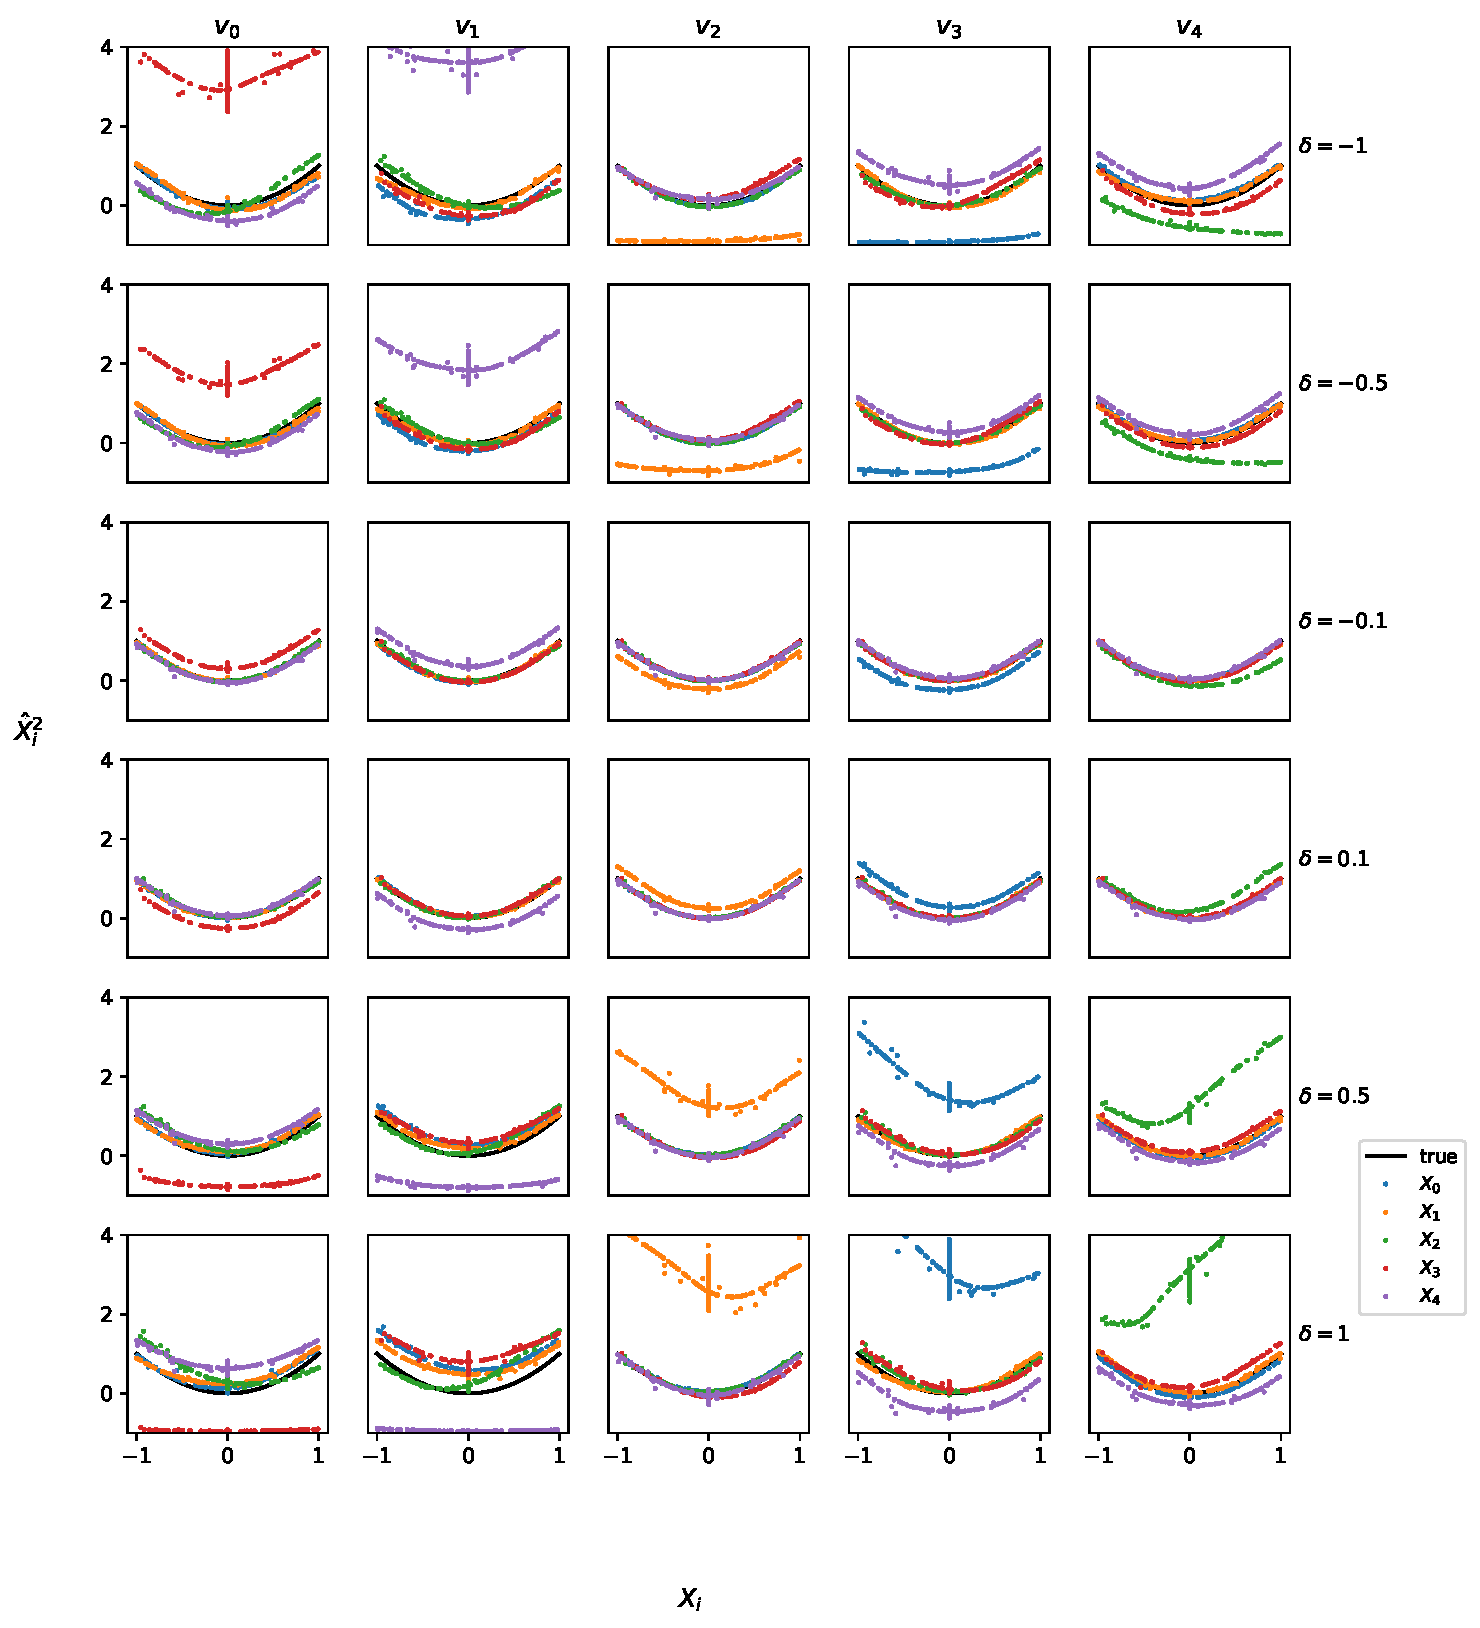
\includegraphics[width=\textwidth]{../figures/s7_squared_intervention_more_deltas.pdf}}
    \centering
    \caption{Effects of intervening on each of the 5 subnetworks of the $X \mapsto X^2$ model.}\label{fig:s7_squared_intervention_more_deltas}
\end{figure}

%--------------------- FIGURE S8: Squared Model Middle Layer Intervention ---------------------
\begin{figure}[ht]
    \centerline{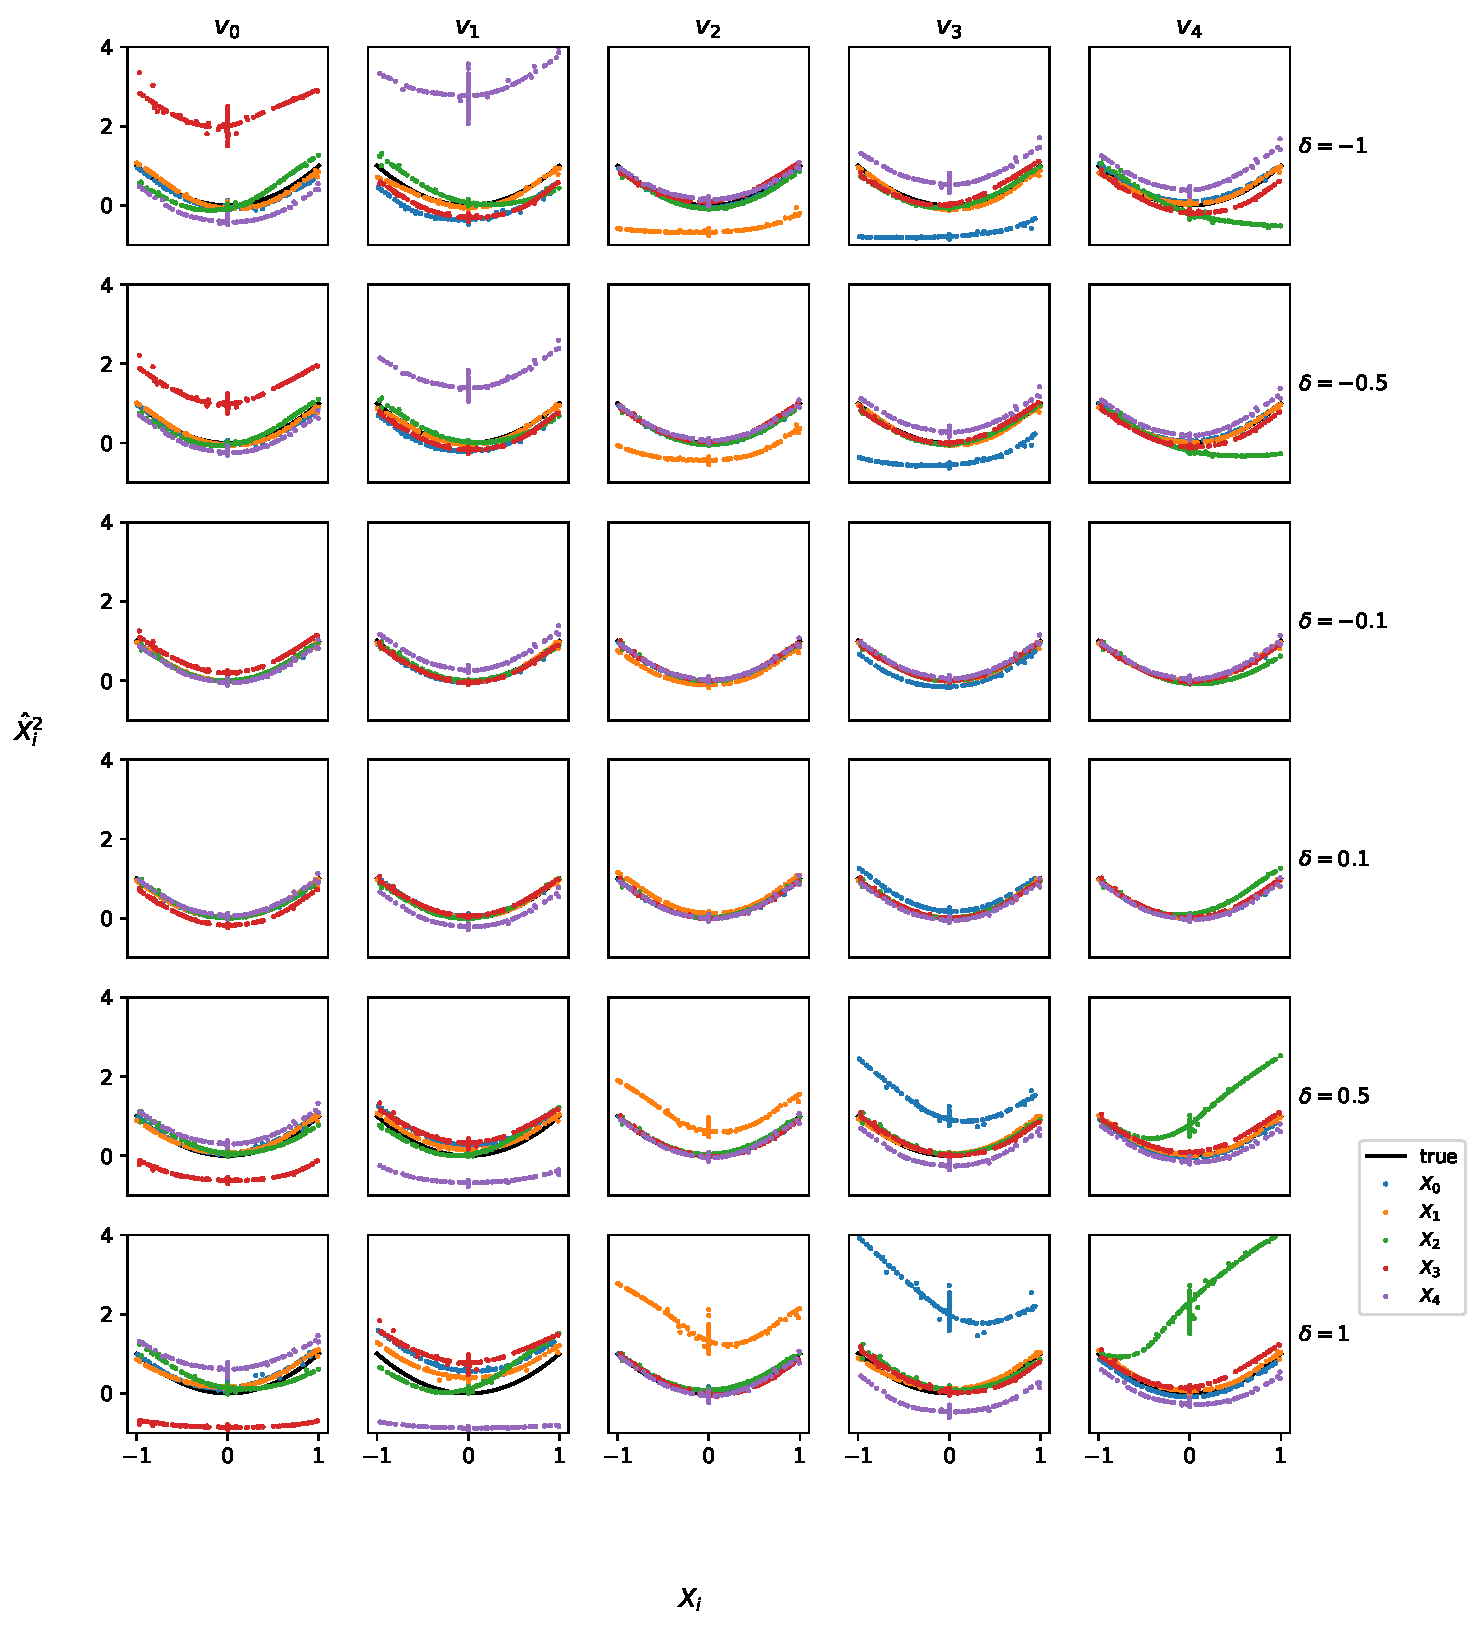
\includegraphics[width=\textwidth]{../figures/s8_squared_intervention_middle_weights.pdf}}
    \centering
    \caption{Intervening on just the weights and biases of the middle hidden layers in the $X \mapsto X^2$ network.}\label{fig:s8_squared_intervention_middle_weights}
\end{figure}


%--------------------- FIGURE S9: Squared Model Multi-Feature Intervention ---------------------
\begin{figure}[ht]
    \centerline{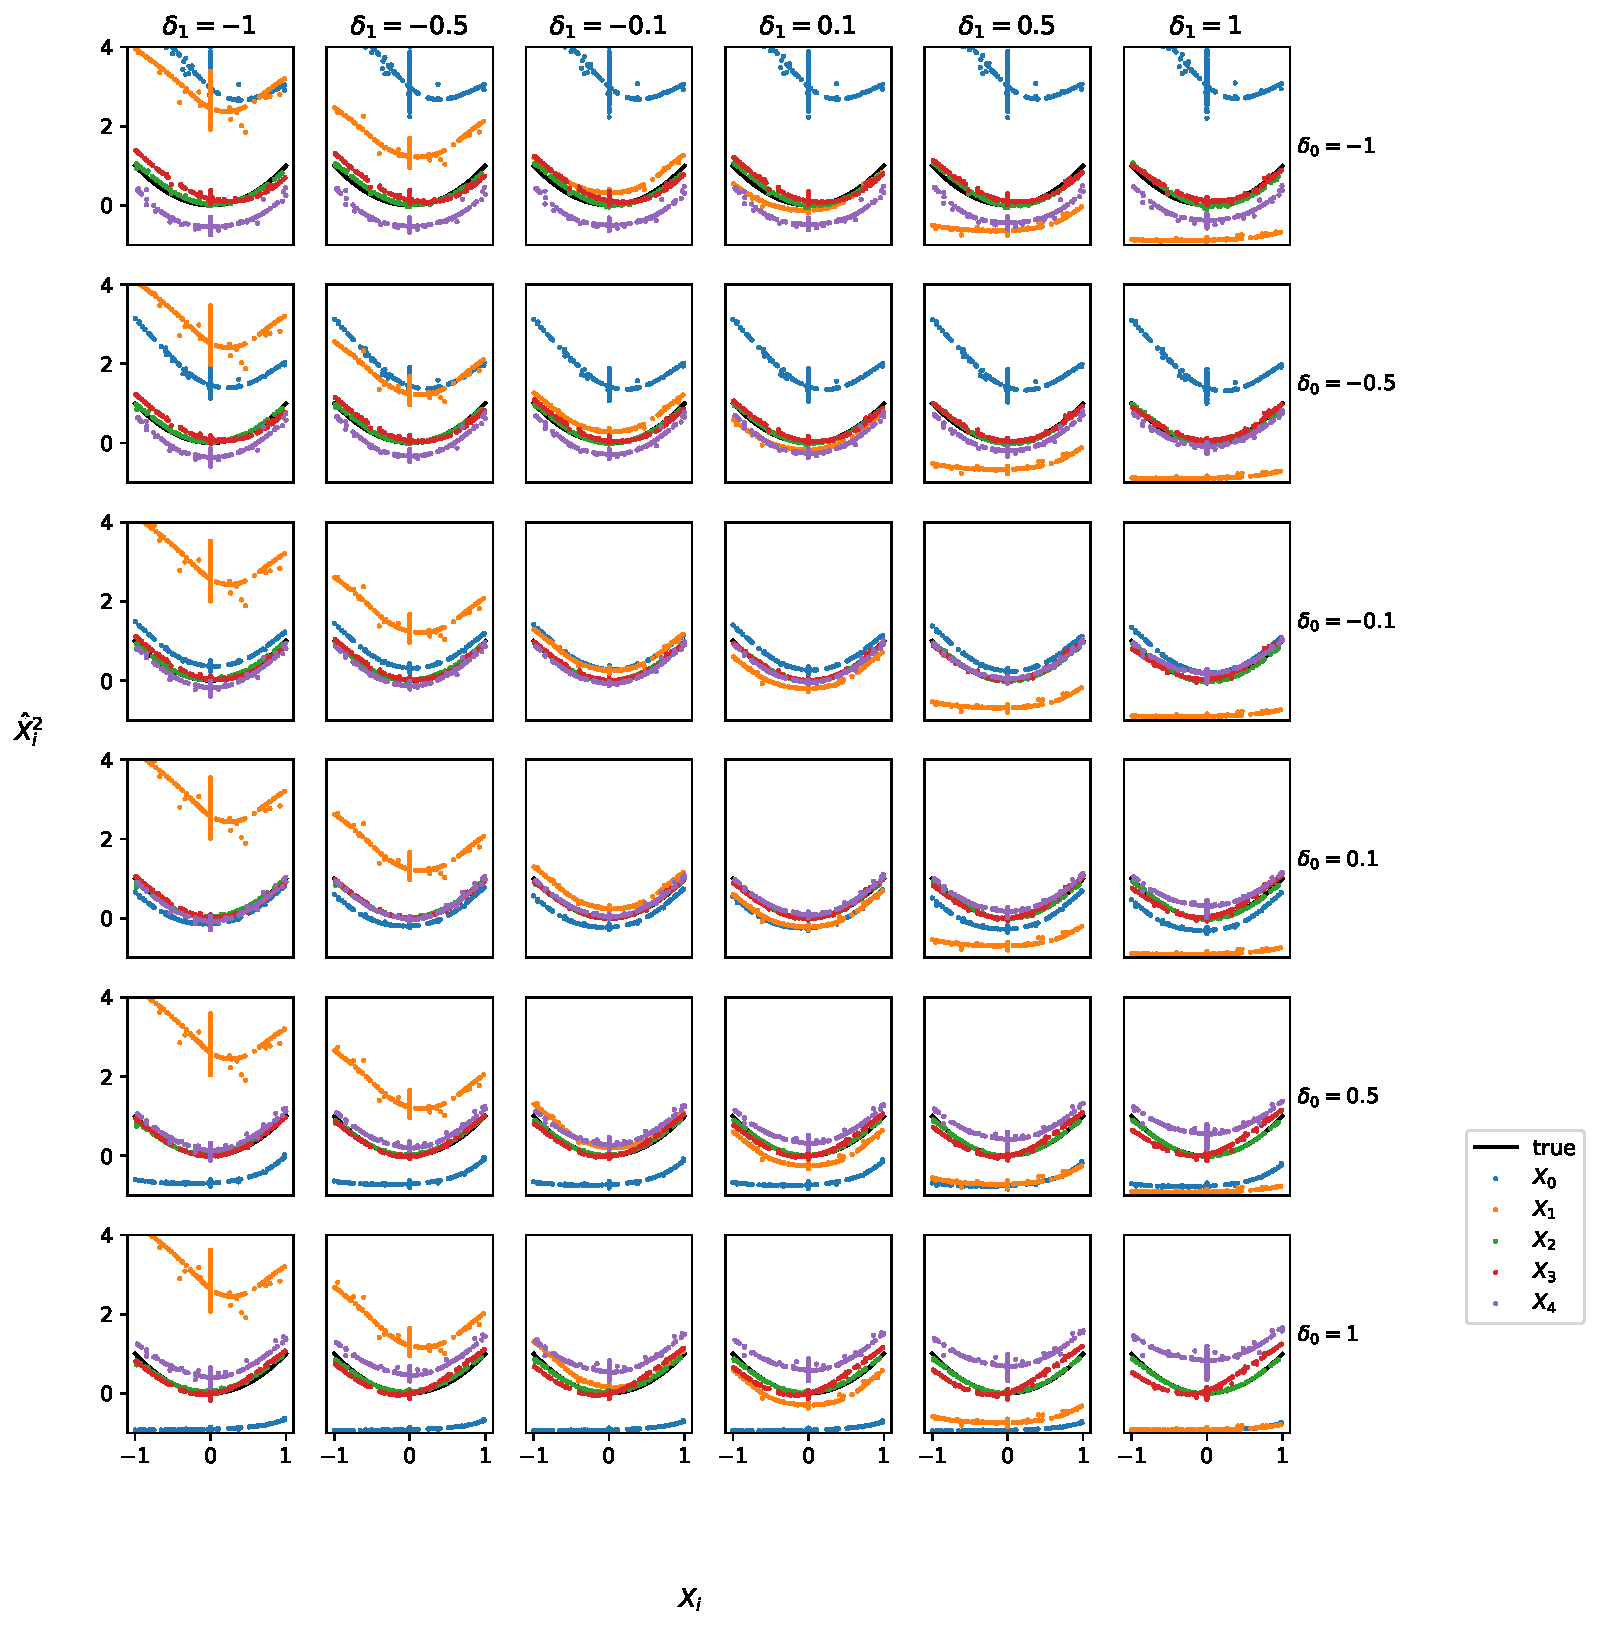
\includegraphics[width=\textwidth]{../figures/s9_squared_intervention_multi_features.pdf}}
    \centering
    \caption{Intervening on multiple subnetworks at once.}\label{fig:s9_squared_intervention_multi_features}
\end{figure}

%--------------------- FIGURE S10: Squared Model Decompositions ---------------------

% rootate this figure to landscape

\begin{figure}[ht]
    \centering
    \caption{Decomposing the $X \mapsto X^2$ model into different numbers of subnetworks}\label{fig:s10_squared_decompositions_features}
    \begin{minipage}{\textwidth} % Ensure figures align
        \centering
        \begin{tabular}{c}  % 3 columns
            \begin{subfigure}{0.3\textwidth}
                \centering
                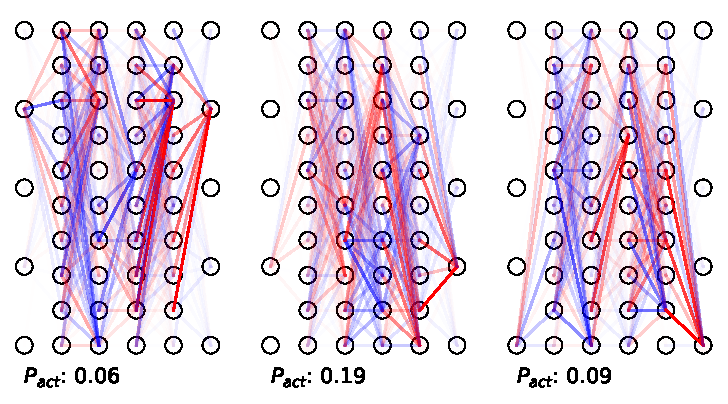
\includegraphics[width=\linewidth]{../figures/s10_squared_decompositions_feature3.pdf}
                \caption{3 rank-1 Networks}
            \end{subfigure} \\
            \begin{subfigure}{0.3\textwidth}
                \centering
                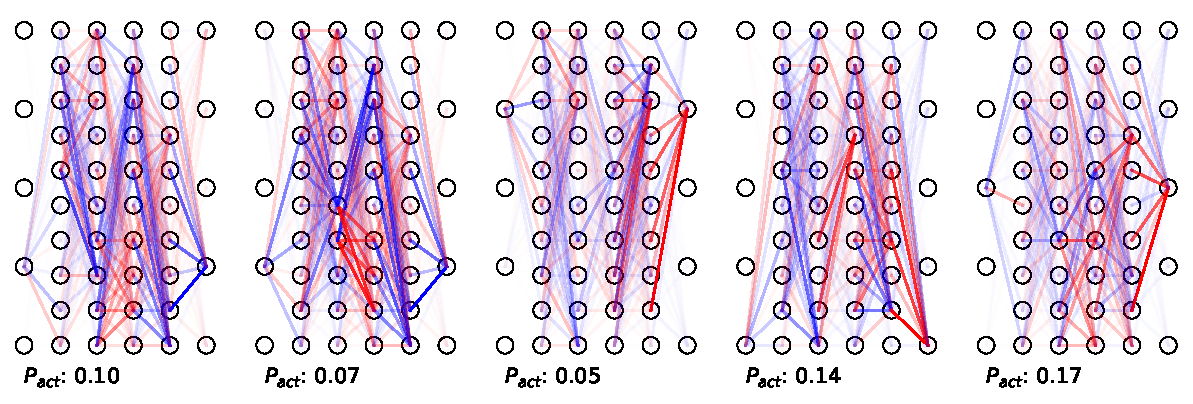
\includegraphics[width=\linewidth]{../figures/s10_squared_decompositions_feature5.pdf}
                \caption{5 rank-1 Networks}
            \end{subfigure} \\ % Move to the next row
            \begin{subfigure}{0.3\textwidth}
                \centering
                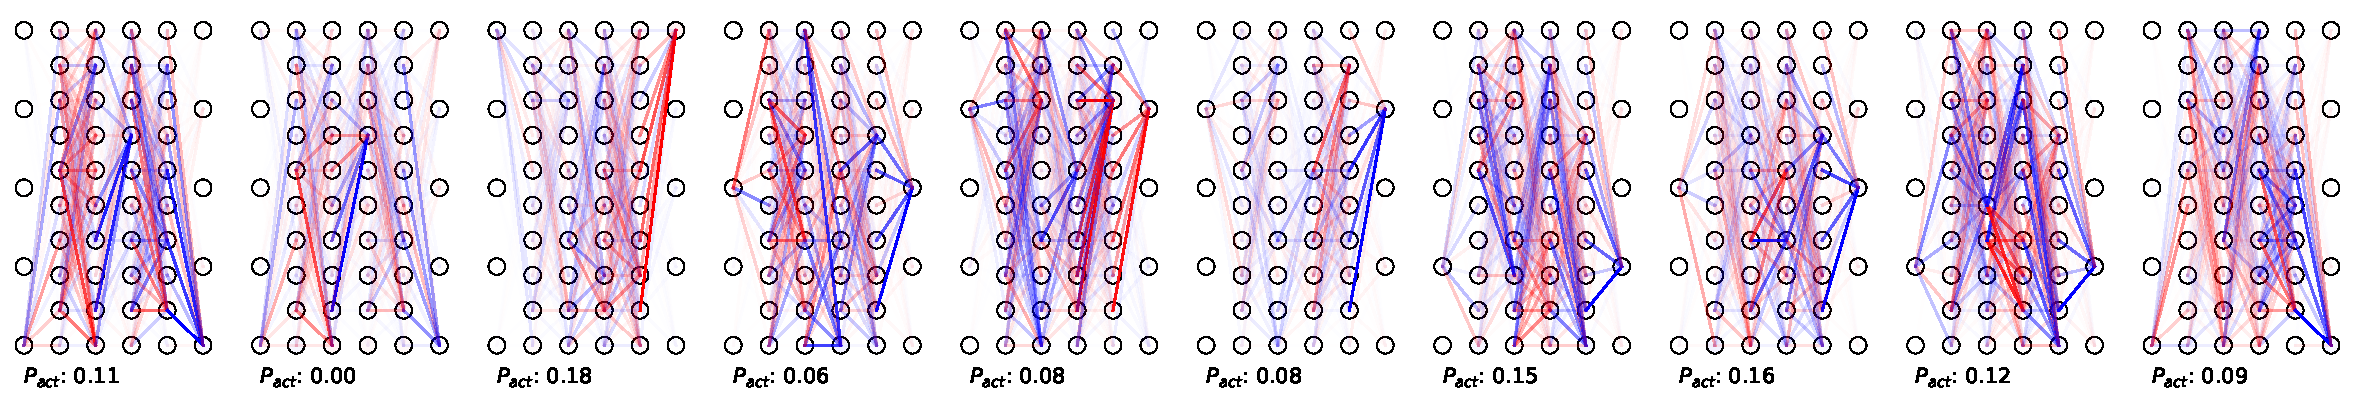
\includegraphics[width=\linewidth]{../figures/s10_squared_decompositions_feature10.pdf}
                \caption{10 rank-1 Networks}
            \end{subfigure} \\ % Move to the next row
            \begin{subfigure}{0.3\textwidth}
                \centering
                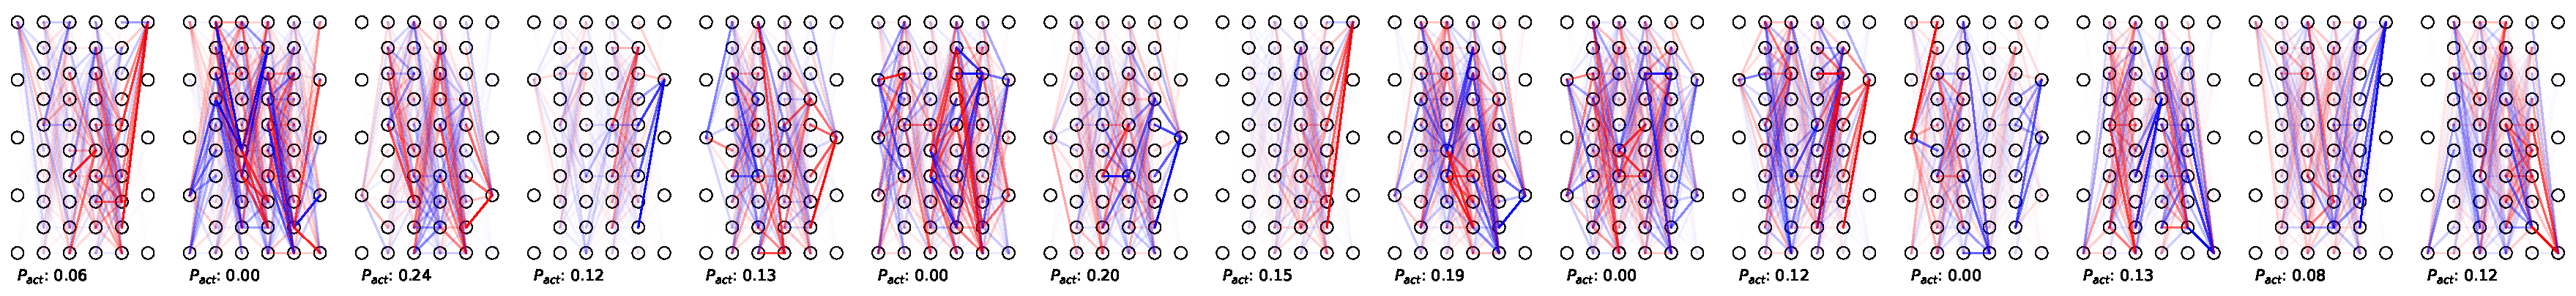
\includegraphics[width=\linewidth]{../figures/s10_squared_decompositions_feature15.pdf}
                \caption{15 rank-1 Networks}
            \end{subfigure} 
        \end{tabular}
    \end{minipage}

\end{figure}

%--------------------- FIGURE S11: Squared Model Loss Versus Rank ---------------------
\begin{figure}[ht]
    \centerline{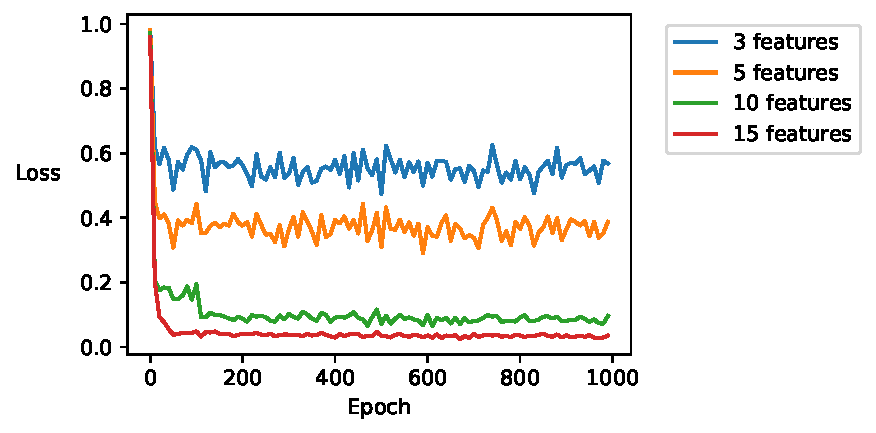
\includegraphics[width=\textwidth]{../figures/s11_squared_features_vs_loss.pdf}}
    \centering
    \caption{Training loss vs number of features for the $X \mapsto X^2$ model, and decompositions for a 3- and 5- subnetwork decomposition.}\label{fig:s11_squared_features_vs_loss}
\end{figure}

\end{document}